\documentclass[a4paper,12pt]{article}
\usepackage[utf8]{inputenc}

\usepackage{amsmath}
\usepackage{amssymb}

\usepackage[T1]{fontenc}
\usepackage[english, polish]{babel}
\usepackage{tikz}
\usetikzlibrary{conceptgraph}
%\DeclareMathSymbol{\vDash}        {\mathrel}{AMSa}{"0F}

\newcommand{\sg}{{\it sg} }
\newcommand{\pl}{{\it pl} }
\newcommand{\mass}{{\it mass} }
\newcommand{\ind}{{\it indexical} }
\newcommand{\corf}{{\it coreferential} }
\newcommand{\deict}{{\it deictic} }
\newcommand{\interr}{{\it interrogative} }

\newcommand{\type}[2]{\text{{\sc type}}(#1,\text{#2})}
\newcommand{\hasName}[2]{\text{{\sc hasName}}(#1,\text{'#2'})}
\newcommand{\dscr}[2]{\text{{\sc dscr}}(#1,#2)}
\newcommand{\init}[2]{\text{{\sc init}}(#1,#2)}
\newcommand{\thme}[2]{\text{{\sc thme}}(#1,#2)}
\newcommand{\thmeGoal}[2]{\text{{\sc thmeGoal}}(#1,#2)}
\newcommand{\expr}[2]{\text{{\sc expr}}(#1,#2)}
\newcommand{\poss}[2]{\text{{\sc poss}}(#1,#2)}
\newcommand{\attr}[3]{\text{{\sc attr}}(#1,#2,#3)}
\newcommand{\attrGoalB}[3]{\text{{\sc attrGoal}}_{#3}(#1,#2)}
\newcommand{\attrB}[3]{\text{{\sc attr}}_{#3}(#1,#2)}
\newcommand{\attrBX}[4]{\text{{\sc attr}}_{#4}(#1,#2,#3)}
\newcommand{\attrA}[2]{\text{{\sc attr}}(#1,#2)}
\newcommand{\manr}[3]{\text{{\sc manr}}(#1,#2,#3)}
\newcommand{\manrA}[2]{\text{{\sc manr}}(#1,#2)}
\newcommand{\prtc}[2]{\text{{\sc prtc}}(#1,#2)}
\newcommand{\pres}[1]{\text{{\sc pres}}(#1)}
\newcommand{\past}[1]{\text{{\sc past}}(#1)}
\newcommand{\fut}[1]{\text{{\sc fut}}(#1)}
\newcommand{\indexic}{\text{{\sc indexical}}}
\newcommand{\deictic}{\text{{\sc deictic}}}
\newcommand{\coreferential}{\text{{\sc coreferential}}}
\newcommand{\loc}[3]{\text{{\sc loc}}(#1,#2,#3)}
\newcommand{\locsrc}[3]{\text{{\sc locSrc}}(#1,#2,#3)}
\newcommand{\locgoal}[3]{\text{{\sc locGoal}}(#1,#2,#3)}
\newcommand{\path}[3]{\text{{\sc path}}(#1,#2,#3)}
\newcommand{\locA}[2]{\text{{\sc loc}}(#1,#2)}
\newcommand{\locsrcA}[2]{\text{{\sc locSrc}}(#1,#2)}
\newcommand{\locgoalA}[2]{\text{{\sc locGoal}}(#1,#2)}
\newcommand{\pathA}[2]{\text{{\sc path}}(#1,#2)}
\newcommand{\meas}[2]{\text{{\sc measure}}(#1,#2)}
\newcommand{\equal}[3]{\text{{\sc equal}}(#1,#2,#3)}
\newcommand{\cref}[2]{\text{{\sc coref}}(#1,#2)}
\newcommand{\crefB}[3]{\text{{\sc coref}}_{#3}(#1,#2)}
\newcommand{\cntA}[2]{\text{{\sc count}}(#1,#2)}
\newcommand{\cnt}[3]{\text{{\sc count}}(#1,#2,#3)}
\newcommand{\tmeA}[2]{\text{{\sc time}}(#1,#2)}
\newcommand{\tme}[3]{\text{{\sc time}}(#1,#2,#3)}
\newcommand{\scc}[2]{\text{{\sc succ}}(#1,#2)}
\newcommand{\dur}[3]{\text{{\sc dur}}(#1,#2,#3)}
\newcommand{\cond}[3]{\text{{\sc cond}}(#1,#2,#3)}
\newcommand{\purp}[3]{\text{{\sc purp}}(#1,#2,#3)}

\title{Kategorialny Parser Składniowo-Semantyczny „ENIAM”\\{\Large definicja reprezentacji semantycznej}}
\author{Wojciech Jaworski}
\date{}

\begin{document}

\maketitle
 
\section{Wprowadzenie}

Znaczenie wypowiedzeń reprezentowane jest w systemie dwupoziomowo.
Najpierw za pomocą grafu semantycznego opisującego występujące w tekście pojęcia
oraz związki pomiędzy nimi a następnie w postaci formuły logiki pierwszego rzędu
rozszerzonej o predykat metajęzykowy i dodatkowe kwantyfikatory.

Następne trzy sekcje niniejszego dokumentu opisują poglądowo poszczególne elementy formalizmu,
po nich następuje teoriomodelowa definicja.

%TODO
% Różnica pomiędzy reprezentacjami polega na tym, że
% graf semantyczny jest bliższy składni, natomiast formuła logiczna posiada formalnie zdefiniowaną semantykę.
% Formuła logiczna jest generowana z grafu semantycznego za pomocą algorytmu, co pozwala przenieść
% formalną semantykę na graf. Niniejszy dokument skupia się na opisie poszczególnych zjawisk językowych za pomocą grafów semantycznych.

Grafy semantyczne inspirowane są pracami Johna Sowy „Knowledge Representation:
Logical, Philosophical, and Computational Foundations”

%TODO
% Podstawy reprezentacji zostały opracowane w ramach projektu Clarin i
% są opisane w dokumencie: ``Język reprezentacji znaczenia dla języka
% polskiego'' oraz szkicowo opublikowane na konferencji COLING 2016 w 
% pracy ``ENIAM: Categorial Syntactic-Semantic Parser for Polish''.
% Poniżej zostanie opisane sposób w jaki poszczególne zjawiska składniowe 
% są reprezentowane za pomocą grafów pojęć. Opis ma charakter techniczny 
% i nie obejmuje rozważań dotyczących teoriomodelowej semantyki poszczególnych konstrukcji, 
% analizy możliwych reprezentacji ani kontekstów literaturowych. 
% Celem, oprócz opisania zasad tworzenia form logicznych przez parser ENIAM
% jest określenie formatu zasobów leksykalnych potrzebnych do ich wygenerowania.

\section{Grafy i formuły}
Formuły naszego języka reprezentacji znaczenia wyrażamy graficznie
w formie grafów semantycznych. % równoważnych tradycyjnie rozumianym formułom logicznym.
Przykładowo dla zdania {\it Słoń trąbi} uzyskamy graf: 

\[\begin{tikzpicture}
\node[concept] (t) {trąbić};
\node[relation, right=1cm of t] (ts) {Init};
\node[concept, right=1cm of ts] (s) {\sg słoń};
\node[relation, left=1cm of t] (pr) {Pres};
\context{cx}{(t)(ts)(s)}{};
\edge {t} {ts};
\edge {cx} {pr};
\edge {ts} {s};
\end{tikzpicture}\]

W powyższym grafie pudełka reprezentują byty, o których jest mowa.
Występuje zatem obiekt {\it słoń} i zdarzenie {\it trąbić}.
Symbol $\sg$ określa liczność obiektów jako dokładnie 1.
Występujące w pudełkach napisy to typy bytów, są nimi pochodzące ze Słowosieci sensy.\footnote{Formalnie sensy w Słowosieci identyfikują leksemy zaopatrzone 
w numery rozpoznające poszczególne znaczenia, np {\it słoń 1} i {\it trąbić 1}. Aby zwiększyć czytelność prezentacji będziemy jednak konsekwentnie 
pomijać te numery.}

Kółeczka zawierają nazwy ról tematycznych opisujących powiązania pomiędzy bytami.
Init wskazuje na to, że {\it słoń} jest inicjatorem {\it trąbienia},
a Pres na to, że zdarzenie jest równoczesne z czasem jego wypowiedzenia.
Źródłem informacji o rolach tematycznych argumentów czasowników 
(a w przyszłości również rzeczowników, przymiotników i przysłówków) jest słownik walencyjny Walenty.

Zewnętrzna ramka to kontekst. Reprezentuje on sytuację, czyli 
podzbiór czasoprzestrzeni, w którym istnieją byty wskazane przez pojęcia w pudełkach
i zachodzą wymienione w kółeczkach związki pomiędzy nimi.

Powyższy graf jest równoważny formule logicznej
\[\exists(x,\dscr{x}{\exists(s,\type{s}{słoń}\wedge|s|=1,\]\[\exists(t,\type{t}{trąbić}\wedge\init{t}{s}))},\pres{x}),\]
w której każdy z obiektów jest identyfikowany przez zmienną.
Predykat $\type{x}{t}$ przypisuje typ t do zmiennej $x$,
to znaczy, stwierdza, że zbiór bytów wskazywanych 
przez $x$ należy do sensu t.
Ze zmiennymi zawsze wiążemy zbiory bytów. Pozwala to w prosty sposób zdefniować zdefiniować liczność.
Predykaty {\sc init} i {\sc pres} odpowiadają rolom tematycznym.
Z kolei predykat metajęzykowy {\sc dscr} wyraża kontekst.

Standardowo każdej jednostce leksykalnej (leksemowi lub wyrażeniu wielosłownemu) 
zawartej w zdaniu odpowiada pudełko, a relacji składniowej kółeczko.
Pudełka zawierają sensy jednostek leksykalnych. Mogą też zawierać ich liczbę i/lub kwantyfikację. 
Zaś w przypadku nazw własnych nazwę i typ nazwy własnej np {\it Franciszek trąbi}:
\[\begin{tikzpicture}
\node[concept] (t) {trąbić};
\node[relation, right=1cm of t] (ts) {Init};
\node[concept, right=1cm of ts] (s) {\sg osoba ``Franciszek''};
\node[relation, left=1cm of t] (pr) {Pres};
\context{cx}{(t)(ts)(s)}{};
\edge {t} {ts};
\edge {cx} {pr};
\edge {ts} {s};
\end{tikzpicture}\]
Formuła odpowiadająca temu zdaniu ma postać
\[\exists(x,\dscr{x}{\exists(o,\type{o}{osoba}\wedge\hasName{o}{Franciszek}\wedge|o|=1,\]\[\exists(t,\type{t}{trąbić}\wedge\init{t}{o}))},\pres{x}).\]
Nazwy własne reprezentujemy za pomocą predykatu $\hasName{x}{name}$, który wiąże 
nazwę 'name' ze zbiorem bytów oznaczonym przez $x$.
W grafach semantycznych nazwy własne (np. {\it Franciszek}) umieszczamy w cudzysłowach.
Nazwy własne nie definiują typu obiektu, tylko identyfikują obiekt poprzez podanie przypisanej mu etykiety.

Poszczególne elementy obu formalizmów reprezentacji znaczenia opiszemy szczegółowo w następnych rozdziałach.

\section{Składnia powiązań między pojęciami}
Związki pomiędzy pojęciami reprezentujemy za pomocą kułeczek zaopatrzonych w strzałki wskazujące charakter udziału
każdego z pojęć w związku. W notacji logicznej kułeczkom odpowiadają predykaty a strzałki wskazują ich argumenty.
Kierunek strzałek w relacjach jest określony tak, by prowadziły od pojęcia stanowiącego nadrzędnik w
drzewie zależności składniowych do pojęcia stanowiącego podrzędnik w tym drzewie\footnote{Jest to ogólna reguła, która ma zastosowanie,
gdy relacja semantyczna wiąże pojęcia odpowiadające słowom połączonym związkiem składniowym. W konkretnych sytuacjach mogą się 
pojawiać wyjątki od niej.}.
Zabieg ten ma na celu zwiększenie czytelności grafów.
Występuje 5 układów strzałek. 
Poniższy graf semantyczny dla zdania {\it Piłka leży pod stołem} prezentuje trzy z nich:
\[\begin{tikzpicture}
\node[concept] (a) {leżeć};
\node[relation, left=1cm of a] (b) {Thme};
\node[concept, left=1cm of b] (c) {\sg piłka};
\node[relation, above=0.8cm of a] (d) {Pres};
\node[relation, right=1cm of a] (e) {Loc};
\node[concept, right=1cm of e] (f) {pod};
\node[concept, below=5mm of e] (h) {\sg stół};
\context{cx}{(a)(b)(c)(e)(f)(h)}{};
\edge {a} {b};
\edge {b} {c};
\edge {cx} {d};
\edge {a} {e};
\edge [dashed]{e} {f};
\edge {e} {h};
\end{tikzpicture}\]
Są to: 
\begin{itemize}
\item jednoargumentowa rola Pres, strzałka wskazująca argument prowadzi do kółeczka;
\item dwuargumentowa rola Thme, strzałka wchodząca do kółeczka jest pierwszym argumentem, a strzałka wychodząca drugim;
\item trójargumentowa rola Loc, strzałka wchodząca do kółeczka jest pierwszym argumentem, przerywana strzałka wychodząca drugim, a ciągła wychodząca trzecim.
\end{itemize}
Zdanie {\it Słoń stał się różowy} prezentuje przykład czwartego typu:
\[\begin{tikzpicture}
\node[concept] (a) {stać się};
\node[relation, left=1cm of a] (d) {Past};
\node[relation, right=1cm of a] (e) {Attr};
\node[concept, below=0.5cm of e] (f) {\sg słoń};
\node[relation, below=0.5cm of a] (g) {Thme};
\node[concept, right=1cm of e] (h) {różowy};
\context{cx}{(a)(e)(f)(g)(h)}{};
\edge {cx} {d};
\edge[dashed] {a} {e};
\edge {f} {e};
\edge {a} {g};
\edge {e} {h};
\edge {g} {f};
\end{tikzpicture}\]
Jest to:
\begin{itemize}
\item parametryzowana przez zdarzenie dwuargumentowa rola Attr, gdzie ciągła strzałka wchodząca do kółeczka jest pierwszym argumentem, wychodząca wychodząca drugim, a przerywana wchodząca wskazuje parametryzujące zdarzenie.
\end{itemize}
Piąty typ występujący w zdaniu {\it Książka jest o grzybach} stanowi połączenie typu trzeciego i czwartego:
\[\begin{tikzpicture}
\node[concept] (a) {być};
\node[relation, left=1cm of a] (d) {Pres};
\node[relation, right=1cm of a] (e) {Attr};
\node[concept, below=0.5cm of e] (f) {\sg książka};
\node[relation, below=0.5cm of a] (g) {Thme};
\node[concept, right=1cm of e] (h) {o};
\node[concept, above=5mm of e] (j) {\pl grzyb};
\context{cx}{(a)(e)(f)(g)(h)(j)}{};
\edge {cx} {d};
\edge[dashed] {a} {e};
\edge {f} {e};
\edge {a} {g};
\edge [dashed]{e} {h};
\edge {g} {f};
\edge {e} {j};
\end{tikzpicture}\]
Mamy tu:
\begin{itemize}
\item parametryzowaną przez zdarzenie trójargumentową rolę Attr, strzałka wchodząca do kółeczka jest pierwszym argumentem, przerywana strzałka wychodząca drugim, ciągła wychodząca trzecim, a przerywana wchodząca wskazuje parametryzujące zdarzenie.
\end{itemize}

\section{Role tematyczne w „Walentym”}
Zbiór ról tematycznych jest rozszerzeniem systemu ról tematycznych ze
słownika walencyjnego „Walenty”. Poniżej prezentujemy listę ról wraz z ich definicjami 
wziętymi z „Zasad opracowania ram semantycznych w słowniku
walencyjnym Walenty” autorstwa Anny Andrzejczuk i Elżbiety Hajnicz.
Skróty nazw ról są inspirowane skrótami zaproponowanymi przez
Johna Sowę w książce „Knowledge Representation”.
Role występujące w systemie Walentego dzielimy na podstawowe
opisujące obligatoryjnych uczestników sytuacji:
\begin{description}
\item{Initiator (Init)} ktoś, kto lub coś, co inicjuje czynność wskazaną przez predykat akcji;
\item{Stimulus (Stim)} coś lub ktoś, kto swoją cechą, właściwością wywołuje reakcję w Experiencerze;
\item{Theme (Thme)} ktoś lub coś, kto lub co podlega działaniu Initiatora, jakiemuś samoistnemu procesowi lub znajduje się w jakimś stanie;
\item{Experiencer (Expr)} ktoś odczuwający uczucia, emocje, przeżywający różne stany psychiczne, mimowolnie odbierający bodźce zmysłami;
\item{Factor (Fctr)} ktoś, kto choć bezpośrednio nie wykonuje danej czynności, to przyczynia się w sposób czynny do jej wykonania, ma wpływ na sytuację, wspomaga, a nawet umożliwia jej zaistnienie;
\item{Instrument (Inst)} coś, dzięki czemu możemy wykonać jakąś czynność, co pełni funkcję wspomagającą, ułatwiającą wykonanie akcji;
\item{Recipent (Rcpt)} ktoś, ku komu jest skierowana czynność, ale kto tej czynności nie podlega, do kogo jest skierowana wypowiedź, z myślą o kim podejmowana jest akcja;
\item{Result (Rslt)} coś, co jest efektem końcowym akcji, na którą wskazuje predykat, co powstaje w jej wyniku.
\end{description}
Oprócz tego rozważane są role uzupełniające, które służą do reprezentacji charakteru okoliczności sytuacji:
\begin{description}
\item{Measure (Meas)} przypisujemy argumentom, które informują w jakim stopniu została wykonana czynność czy
jaka jest jej wielkość, a dokładniej podają miarę tej czynności;
\item{Location (Loc)} określa miejsce, w którym dzieje się akcja czy też skąd lub dokąd zmierza uczestnik sytuacji;
\item{Path (Path)} to trasa, ścieżka, droga, czy to w sensie fizycznym, metafizycznym czy metaforycznym;
\item{Time (Time)} to czas, w którym coś się dzieje;
\item{Duration (Dur)} określa czas trwania sytuacji, na którą wskazuje predykat;
\item{Condition (Cond)} określa okoliczności, bez zaistnienia których nie doszłoby do zaistnienia akcji; informuje o przyczynie lub warunkach zaistnienia sytuacji;
\item{Purpose (Purp)} określa cel, który przyświeca sytuacji, na którą wskazuje predykat; gdyby Initiatorowi nie przyświecał ten cel, nie doszłoby do danej sytuacji; określa też nasze marzenia, życzenia, oczekiwania.
\item{Attribute (Attr)} jako jedyna z ról uzupełniających określa jednego z uczestników sytuacji; przypisujemy ją
cechom, właściwościom ludzi, zwierząt, przedmiotów, zjawisk, procesów, a także stanom, emocjom itp;
\item{Manner (Manr)} określa, w jaki sposób została wykonana określona czynność;
\end{description}
Powyższy zbiór ról modyfikowany jest rolami pomocniczymi --- atrybutami ról.
Role pomocnicze służą rozróżnieniu uczestników sytuacji, którzy mają tą samą rolę podstawową lub uzupełniającą.

Rolę główną opatrujemy atrybutami Foreground, Background, gdy w ramie semantycznej
istnieją dwa argumenty mające przypisaną tę rolę. Podstawą do przypisania tych atrybutów, 
jest równorzędność argumentów opatrzonych tą rolą.

Rolę główną opatrujemy atrybutami Source, Goal wówczas, gdy oba argumenty pełnią taką samą rolę
w zdaniu, ale sytuacja wskazuje kierunek wykonywanej czynności czy procesu. Source (Src) to początek, 
źródło procesów, czynności, a Goal (Goal) to cel, do którego się dąży lub etap końcowy procesu, czynności.
Wyjątek stanowi tu rola Location, gdzie Location Source informuje o miejscu początkowym czynności a Location Goal o miejscu końcowym.

W naszym systemie znaczenie roli Measure jest rozszerzone na rzeczowniki i oznacza ona miarę dla pojęć wyrażonych przez rzeczowniki niepoliczalne.
Oprócz niej wprowadzamy rolę Count wyrażającą liczebność odniesienia rzeczoników policzalnych.

Jednoargumentowe role Past, Pres i Fut wskazują związek czasu wypowiedzi z czasem, do którego się ona odnosi.
Z kolei rola Successor (Succ) wyraża następstwo czasowe sytuacji.

\section{Model}
Zdefniujemy teraz model, w którym będziemy wyrażać formalną semantykę naszych języków reprezentacji znaczenia.
Semantykę zdefiniujemy wpierw dla formuł logicznych, nastepnie w rozdziale \ref{mrs} przeniesiemy jej definicję na grafy semantyczne.

Dla osób nieobeznanych z logiką formalną: 
Model możemy sobie wyobrażać jako strukturę danych, która zawiera przecyzyjny opis tego 
co znajduje się w świecie, informacje o wszystkich bytach i relacjach między nimi.
Grafy pojęć i formuły logiczne stanowią teorię opisującą ten model.
Model również opisujemy za pomocą pewnego formalizmu (języka),
więc na pierwszy rzut oka treść tego rozdziału może wydawać się „tłumaczeniem z polskiego na nasze”.
Tym niemniej istnieje fundamentalna różnica między modelem a opisującą go teorią:
model wyraża dokładnie to co jest, a teoria zawiera zbiór zdań, które w tym modelu są prawdziwe.
Zatem kompletny opis modelu jest (często nieskończonym) zbiorem predykatów stwierdzającym 
co w modelu jest prawdziwe. W opisie tym nie ma miejsca na negację, alternatywę, czy implikację.
Z kolei od teorii wymagamy jedynie tego by była zgodna z modelem, czyli prawdziwa, nie musi ona być kompletna.

%TODO: uporządkować kwestię funkcja/relacja/atrybut
%TODO: uporządkować kwestię model/sytuacja
Model $\cal M$ jest to uniwersum, czyli zbiór wszystkich bytów, oraz zależne od czasu relacje i 
funkcje zdefiniowane na tych bytach. Niech $x$ będzie elementem uniwersum modelu, który jest w relacji $r$ z elementem $y$ w chwili $t$.
Fakt ten będziemy oznaczać $x.r(t)=y$. Notacja ta odzwierciedla przyjęte przez nas rozumienie 
funkcji i relacji jako cech (atrybutów) bytów. Tak więc $r$ jest cechą, atrybutem $x$, a $y$ jest wartością tej cechy.
Jeśli dany atrybut nie zmienia swojej wartości w przeciągu sytuacji opisywanej przez model argument czasowy pomijamy w notacji,
tzn. zamiast $x.r(t)=y$ napiszemy $x.r=y$.

Wśród elementów uniwersum znajdują się 
\begin{itemize}
\item liczby,
\item interwały, czyli odcinki czasu,
\item zdarzenia i stany,
\item przedmioty,
\item napisy,%TODO: to trzeba by czymś zastąpić np. sekwencja zapisanych lub wypowiedzianych dźwięków???
\item sytuacje,
\item algorytmy znaczeniowe.
\end{itemize}

Przykładowe atrybuty to 
\begin{description}
\item $beg$ wiążący interwał z punktem w czasie będącym jego początkiem, 
\item $end$ wiążący interwał z punktem w czasie będącym jego końcem, 
\item $len$ wskazujący długość interwału.
\item $time$ oznaczający czas zdarzenia/stanu, 
\item $loc$ oznaczający miejsce zdarzenia/stanu/przedmiotu, %parametryzowane przez czas
\item $name$ wiążący byt z napisem będącym jego nazwą.
\end{description}

Interpretacja jest funkcją, która wiąże symbole języka z elementami modelu.
Interpretacja stałej $a$ to element uniwersum, który wskazuje ta stała.
Element ten oznaczany jako $a^{\cal M}$.
Przyjmujemy ponadto, że interpretacją napisu jest on sam,
czyli $s^{\cal M}=s$, gdy $s$ jest napisem.

Zmienne w przeciwieństwie do stałych nie mają interpretacji tylko wartościowanie.
Wartościowanie jest funkcją przypisującą zmiennym elementy uniwersum.
Wartościowanie pozwala zdefniować kwantyfikatory, np formuła $\exists(x,\varphi(x))$ jest
spełniona w modelu ${\cal M}$, gdy istnieje wartościowanie $v$ przypisujące zmiennej $x$
element uniwersum taki, że $\varphi(x)$ jest prawdziwe w modelu ${\cal M}$.

Interpretacją predykatu $p$ jest relacja oznaczana $p^{\cal M}$.
Na przykład interpretacją predykatu {\sc hasName} jest relacja $\text{\sc hasName}^{\cal M}$. 
W naszym modelu przyjmujemy, że $\text{\sc hasName}^{\cal M}=name$. Oznacza to, że 
dla zmiennej $x$ i napisu $s$, formuła $\hasName{x}{s}$ jest prawdziwa wtw.
gdy $v(x).name=s^{\cal M}=s$. 

Prawdziwość formuły $\varphi$ w modelu ${\cal M}$ przy wartościowaniu $v$ wyrażamy za pomocą relacji konsekwencji semantycznej  '$\vDash$'.
Na przykład ostatnie zdanie z poprzedniego akapitu możemy zapisać jako:
\[({\cal M},v\vDash \hasName{x}{s}) \Longleftrightarrow v(x).name=s^{\cal M} \Longleftrightarrow v(x).name=s\]

Predykat {\sc type} wiąże ze sobą zbiór bytów oraz sens ze Słowosieci.
Interpretacjami słowosieciowych sensów są {\it algorytmy znaczeniowe}, 
które dla danego bytu rozstrzygają,
czy można o nich prawdziwie orzec przynależność do sensu.%tę nazwę.
Algorytm znaczeniowy zwraca stałe {\bf True} oraz {\bf False}.
Możemy teraz zdefniować predykat {\sc type}:
\[({\cal M},v\vDash \type{x}{t}) \Longleftrightarrow \text{t}^{\cal M}(v(x))=true\]
Aby uprościć notację zamiast pisać $t(x)={\bf True}$ będziemy pisać $t(x)$,
czyli pozornie utożsamimy wartości zwracane przez algorytmy znaczeniowe 
ze wartościami logicznymi. Ponadto zakładamy, że interpretacja 
danego sensu jest identyczna w każdym modelu, czyli że słowa mają 
ustalone znaczenia wspólne dla wszystkich użytkowników języka. 
Odzwierciedlimy ten fakt w notacji 
oznaczając algorytmy znaczeniowe pogrubioną czcionką i pomijając wskazanie modelu.
Na przykład zamiast pisać $\text{słoń}^{\cal M}$ napiszemy {\bf słoń}.
Zatem powyższą definicję zapiszemy w skrócie jako:
\[({\cal M},v\vDash \type{x}{t}) \Longleftrightarrow \text{{\bf t}}(v(x))\]

\section{Wprowadzanie modelu}
Semantyka języka reprezentacji znaczenia budowana jest na zbiorze możliwych światów.
Przyjmujemy, że każdy mówca prezentuje pewien model świata, w którym interpretuje swoje wypowiedzi i każdy akt komunikacji jest utworzeniem nowego modelu. 
Model ten nazywamy modelem wypowiedzi.
Gdy ktoś coś komunikuje, nie znaczy to, że treść komunikatu jest faktycznie prawdziwa, ani tego, że nadawca wierzy w jej prawdziwość,
a jedynie, że przedstawia model, w którym ona jest prawdziwa.
Dzięki temu, że każdy mówca przedstawia oddzielny model wypowiedzi, reprezentacja semantyczna dłuższego tekstu, 
w którym różne osoby wypowiadają sprzeczne opinie, zdaje z tego sprawę, sama nie będąc kontradyktoryczna.

W sytuacji, w której mówca mówi o tym, co sądził lub co powiedział ktoś drugi, pierwszy symuluje w swoim modelu wypowiedzi model drugiego. 
Może się w tym mylić i wtedy
niezgodność zachodzi między pierwszym modelem a stanem faktycznym świata (tzw. światem aktualnym).
Niezależnie od tego, referowana myśl też może być prawdziwa lub nieprawdziwa -- za to odpowiada już drugi model.

Poszczególne modele mają strukturę hierarchiczną. 
Na przykład zdanie 
\begin{equation}\label{zdanie_Jaswierzy}
\text{Jaś wierzy, że Marysia kłamie, że go nienawidzi.}
\end{equation}
interpretujemy następująco:
\begin{itemize}
\item Na poziomie narracji mamy model ${\cal A}$, w którym zachodzi sytuacja $a$, czyli {\it Jaś wierzy, że ${b}$}.
\item ${\cal B}$ jest modelem, w którym zachodzi sytuacja $b$, czyli {\it Marysia kłamie, że $c$}.
\item ${\cal C}$ jest modelem, w którym zachodzi sytuacja $c$, czyli {\it Marysia nienawidzi Jasia}.
\end{itemize}
{
Zdanie (\ref{zdanie_Jaswierzy}) reprezentowane z użyciem metapredykatu {\sc dscr} będzie miało w ogólności następującą postać 
(reprezentowana jest jedynie zmiana kontekstu):}
\begin{equation}
\begin{array}{c}
\text{{\it Narrator zakomunikował, że }} a \\
\wedge 
\dscr{a}{\text{{\it Jaś wierzy, że }} b} \\
\wedge 
\dscr{b}{\text{{\it Marysia kłamie, że }} c} \\
\wedge 
\dscr{c}{\text{{\it Marysia nienawidzi Jasia}}})))
\end{array}
\end{equation}
% {
% Poniżej reprezentacja uwgzlędniająca znaczenia związków syntaktycznych, czasu gramatycznego, leksykalne i z rozwiązaną koreferencją:}
% \begin{equation}
% \begin{array}{c}
% \dscr{a}{
% \pred{hasName}(j, \text{Jaś}) \wedge
% |j|=1 \wedge
% \type(w, \text{wierzyć})\\ \wedge
% % \pred{praes}(w,t_{1}) \wedge
% % \pred{agent}(w,j) \wedge
% % \pred{topic}(w,b)
% }
% \\
% \wedge \dscr{b}{
% \pred{hasName}(m, \text{Marysia}) \wedge
% |m|=1 \wedge
% \type(k, \text{kłamać})\\ \wedge
% % \pred{past}(k,t_{2}) \wedge
% % \pred{agent}(k,m) \wedge
% % \pred{topic}(k,c)
% }
% \\
% \wedge \dscr{c}{
% \type(n, \text{nienawidzić})\\ \wedge
% % \pred{time}(n,t_{3}) \wedge
% % t_{2} \simeq t_{3}\wedge
% % \pred{agent}(n,m) \wedge
% % \pred{patient}(n,j)
% }
% )))
% \end{array}
% \end{equation}

Z racji tego, że modele mają strukturę hierarchiczną, model wewnętrzny powinien należeć do uniwersum modelu zewnętrznego.
Byty odpowiadające takim modelom nazywamy sytuacjami.
Niech $\varphi$ będzie formułą, a $s$ stałą, której interpretacją w ${\cal M}$ jest sytuacja. Wtedy 
\[({\cal M},v\vDash \dscr{s}{\varphi}) \Longleftrightarrow (v(s).model \vDash \varphi)\]
Atrybut $model$ wiąże sytuację, z opisującym ją modelem.


\section{Wprowadzanie bytów do dyskursu}
W języku logiki pierwszego rzędu wzmiankowane byty stanowią odniesienia zmiennych, a
same zmienne wprowadzane są przez kwantyfikatory. Przy czym dostępne są dwa rodzaje kwantyfikacji:
uniwersalna w której wartościowanie wprowadzanej zmiennej przebiega po wszystkich elementach uniwersum
spełniających restrykcję oraz egzystencjalna, przy której zmienna wartościowana jest jednym 
z bytów spełniających restrykcję.

W przypadku grafów semantycznych zmienne nie są jawnie wskazane, tym niemniej 
zachodzi konieczność określenia w jaki sposób obiekty wskazywane przez pudełka 
są wiązane z uniwersum.

Domyślnie przyjmujemy kwantyfikację egzystencjalną, czyli np. zdanie {\it Słoń trąbi}
stwierdza o istnieniu {\it słonia} i istnieniu zdarzenia {\it trąbienia}.

Z kolei dla zdania {\it Ty biegniesz} otrzymamy reprezentację z pojęciem okazjonalnym (indexical),
który wiąże słowo {\it ty} z uczestnikami komunikacji, czyli odwołuje się do uniwersum na metapoziomie.
\[\begin{tikzpicture}
\node[concept] (t) {biec};
\node[relation, right=1cm of t] (ts) {Init};
\node[concept, right=1cm of ts] (s) {\ind ty};
\node[relation, left=1cm of t] (pr) {Pres};
\context{cx}{(t)(ts)(s)}{};
\edge {t} {ts};
\edge {cx} {pr};
\edge {ts} {s};
\end{tikzpicture}\]
\[\exists(x,\dscr{x}{\exists(s,\type{s}{ty(\#i)},\]\[\exists(t,\type{t}{biec}\wedge\init{t}{s}))},\pres{x}),\]
a dla zdania {\it Ona biegnie} otrzymamy reprezentację z pojęciem deiktycznym 
\[\begin{tikzpicture}
\node[concept] (t) {biec};
\node[relation, right=1cm of t] (ts) {Init};
\node[concept, right=1cm of ts] (s) {\deict ona};
\node[relation, left=1cm of t] (pr) {Pres};
\context{cx}{(t)(ts)(s)}{};
\edge {t} {ts};
\edge {cx} {pr};
\edge {ts} {s};
\end{tikzpicture}\]
\[\exists(x,\dscr{x}{\exists(s,\type{s}{ona(\#d)},\]\[\exists(t,\type{t}{biec}\wedge\init{t}{s}))},\pres{x}),\]
lub koreferencyjnym
\[\begin{tikzpicture}
\node[concept] (t) {biec};
\node[relation, right=1cm of t] (ts) {Init};
\node[concept, right=1cm of ts] (s) {\corf ona};
\node[relation, left=1cm of t] (pr) {Pres};
\context{cx}{(t)(ts)(s)}{};
\edge {t} {ts};
\edge {cx} {pr};
\edge {ts} {s};
\end{tikzpicture}\]
\[\exists(x,\dscr{x}{\exists(s,\type{s}{ona(\#c)},\]\[\exists(t,\type{t}{biec}\wedge\init{t}{s}))},\pres{x}),\]
W powyższych trzech przypadkach nie następuje wprowadzenie nowego bytu do dyskursu. Zmienne wskazujące odniesienia 
pojęć okazjonalnych, deiktycznych i koreferencyjnych są wiązane przez algorytmy znaczeniowe tych pojęć z bytami wskazanymi
przez ich dodatkowe argumenty.

Zaimki wnoszą informację o osobie, liczbie i rodzaju, która jest istotna przy ustalaniu ich referenta.
Z tego tego względu lematyzujemy je do form uwzględniających te informacje ({\it ja}, {\it wy}, {\it one}, {\it która}), ewentualnie uzupełniając 
np. {\it ja-m}.

Operator wprowadzający pojęcie okazjonalne defniujemy następująco:
niech $x$ będzie sytuacją, którą modeluje ${\cal M}$, tzn. $x.model={\cal M}$, wtedy
\[\#i^{\cal M}=x\], czyli 
\[({\cal M},v\vDash \type{s}{ty(\#i)}) \Longleftrightarrow \text{{\bf ty}}(x)(v(s))\]
Algorytmy znaczeniowe dla okazjonalnych zaimków {\it ja} i {\it ty} możemy zdefniować następująco:
\[\text{\bf ja}\equiv\lambda x\lambda y\;x.speaker=y\]
\[\text{\bf ty}\equiv\lambda x\lambda y\;x.hearer=y\]
%TODO: my, wy

% Zaimki indexicalne to wartości cech otaczającej sytuacji, tak jak {\it kolor piłki}

Argument deiktyczny to kontekstowo zdefniowany zbiór $x$ zawierający 
obiekty, na które wskazywał mówca
\[\#d^{\cal M}=x\]
Z kolei argument koreferencyjny to kontekstowo zdefniowany zbiór $x$ zawierający 
obiekty, które były wzmiankowane w wypowiedzi
\[\#c^{\cal M}=x\]
%TODO: skąd te byty się biorą? jakieś inkrementalne otoczenie przenoszone pomiędzy sytuacjami?

Algorytm znaczeniowy zaimka {\it ona} nie zależy od tego czy argument jest koreferencyjny, czy deiktyczny:
\[\text{\bf ona}\equiv\lambda x\lambda y\;y\in x \wedge y.gender=f\]

%TODO: wstawić formuły logiczne
Kiedy podmiot nie jest dany w sposób jawny, jest reprezentowany za pomocą wariantu niemego zaimka {\it pro}
np. {\it Biegnę}.:
\[\begin{tikzpicture}
\node[concept] (t) {biec};
\node[relation, right=1cm of t] (ts) {Init};
\node[concept, right=1cm of ts] (s) {\ind pro-ja};
\node[relation, left=1cm of t] (pr) {Pres};
\context{cx}{(t)(ts)(s)}{};
\edge {t} {ts};
\edge {cx} {pr};
\edge {ts} {s};
\end{tikzpicture}\]
Zaimek {\it pro} używany jest również, kiedy przedmiot jest wprowadzany poprzez podanie swojej cechy, 
co ma miejsce we frazach rzeczownikowych, których głową jest przymiotnik np. {\it Gruby trąbi.}
\[\begin{tikzpicture}
\node[concept] (t) {trąbić};
\node[relation, right=1cm of t] (ts) {Init};
\node[concept, right=1cm of ts] (s) {\ind pro-on};
\node[relation, left=1cm of t] (pr) {Pres};
\node[relation, right=10mm of s] (a) {Attr};
\node[concept, right=1cm of a] (b) {gruby};
\context{cx}{(t)(ts)(s)(a)(b)}{};
\edge {t} {ts};
\edge {cx} {pr};
\edge {ts} {s};
\edge {s} {a};
\edge {a} {b};
\end{tikzpicture}\]
Kolejnym zastosowaniem niemego zaimka są równoważniki zdań.
Dodajemy do nich {\it pro-zdarzenie}, które wiąże poszczególne elementy zdania,
np. {\it Kot pod stołem}
\[\begin{tikzpicture}
\node[concept] (a) {pro-zdarzenie};
\node[relation, left=1cm of a] (b) {Thme};
\node[concept, left=1cm of b] (c) {\sg kot};
\node[relation, above=0.8cm of a] (d) {Pres};
\node[relation, right=1cm of a] (e) {Loc};
\node[concept, right=1cm of e] (f) {pod};
\node[concept, below=0.5cm of e] (h) {\sg stół};
\context{cx}{(a)(b)(c)(e)(f)(h)}{};
\edge {a} {b};
\edge {b} {c};
\edge {cx} {d};
\edge {a} {e};
\edge [dashed]{e} {f};
\edge {e} {h};
\end{tikzpicture}\]
%TODO pro-zdarzenie to może też być stan, przydałaby się ogólniejsza nazwa

W dalszym toku tekstu wprowadzimy jeszcze pojęcia interrogatywne (interrogative),
występujące przy zadawaniu pytań, jak również kwantyfikację uniwersalną 
(przebiegającą po wielu bytach).
%kwantyfikacja uniwesalna może być wprowadzona niejawnie np: Słoń jest ssakiem, 

\section{Definicje podstawowych ról tematycznych}

%TODO !!!
ważyć 


kosztować-2 
Perski dywan kosztował Kalasantego 100.000zł.
Thme                   Recipent    Measure


Jan zaaranżował Marysi spotkanie
Init            Recipent Thme

węszyć-2
Kot węszył za myszami
Expr       Stimulus

golić-2
Kalasanty golił brodę u cyrulika
Thme F          Thme B Factor

Cyrulik ogolił Kalasantemu brodę brzytwą.
Init           Thme F      Thme B Inst

słuchać 


aranżować


\section{Liczebność i miara}

Odniesieniem rzeczowników policzalnych są kolekcje bytów.
Atrybuty kolekcji są jednocześnie atrybutami wszystkich indywiduów wchodzących w jej skład.
W szczególności jednoelementowa kolekcja jest tożsama z indywiduum, które się na nią składa.

Rola Count wskazuje liczebność odniesienia rzeczowników policzalnych
np: {\it Dwa słonie trąbią}, {\it kilka słoni}
\[\begin{tikzpicture}
\node[concept] (t) {trąbić};
\node[relation, right=1cm of t] (ts) {Init};
\node[concept, right=1cm of ts] (s) {słoń};
\node[relation, left=1cm of t] (pr) {Pres};
\node[relation, right=1cm of s] (sk) {Count};
\node[concept, right=1cm of sk] (k) {2};
\context{cx}{(t)(ts)(s)(sk)(k)}{};
\edge {t} {ts};
\edge {cx} {pr};
\edge {ts} {s};
\edge {s} {sk};
\edge {sk} {k};
\end{tikzpicture}\]
\[\exists(x,\dscr{x}{\exists(s,\type{s}{słoń}\wedge\exists(d,\type{d}{dwa},\cntA{s}{d}),\]\[\exists(t,\type{t}{trąbić}\wedge\init{t}{s}))},\pres{x}),\]
lub równoważnie
\[\exists(x,\dscr{x}{\exists(s,\type{s}{słoń}\wedge|s|=2,\]\[\exists(t,\type{t}{trąbić}\wedge\init{t}{s}))},\pres{x}),\]
\[\begin{tikzpicture}
\node[concept] (t) {słoń};
\node[relation, right=1cm of t] (ts) {Count};
\node[concept, right=1cm of ts] (s) {kilka};
\edge {t} {ts};
\edge {ts} {s};
\end{tikzpicture}\]
\[\type{s}{słoń}\wedge\type{k}{kilka}\wedge\cntA{s}{k},\]
Liczebniki odnoszą do liczb i reprezentujemy je jako zmienną desygnującą 
liczbę oraz algorytm znaczeniowy sprawdzający należenie jej  
do zbioru wyznaczonego przez intensję słowa. 
Liczebniki określone reprezentujemy za pomocą liczb, 
a nieokreślone (np {\it kilka, trochę}) za pomocą leksemów.
Algorytmy znaczeniowy dla pojęć {\it 2} i {\it kilka} mają postać 
\[{\bf 2}\equiv \lambda x\; x=2\]
\[{\bf kilka}\equiv \lambda x\; x>2\wedge x<10\]
Predykat {\sc count} zdefiniujemy następująco:
%\[({\cal M},v\vDash \cntA{x}{y}) \Longleftrightarrow |v(x)|= v(y)\]
\[({\cal M},v\vDash \cntA{x}{y}) \Longleftrightarrow v(x).count= v(y)\]
Atrybut $count$ określa liczność kolekcji.
%trzy i pół jabłka jest kolekcją zawierającą 4 elementy: 3 jabłka i jedną połówkę jabłka.

Wprowadzamy też funkcję $|\cdot|$ zwracającą liczność kolekcji:
\[|s|=n\Longleftrightarrow \cntA{s}{n}\]
Dla liczebników określonych wprowadzamy skrót notacyjny:
zamiast wprowadzać zmienną odnoszącą do liczby podajemy wartość tej liczby.
Zatem zamiast pisać 
\[\exists(d,\type{d}{dwa},\cntA{s}{d})\]
napiszemy
\[|s|=2\]


%TODO dokonczyć i porównać z przyimki.tex
Liczebniki mogą być modyfikowane przez operatory adnumeratywne np. {\it prawie 30 słoni}.
\[\begin{tikzpicture}
\node[concept] (t) {słoń};
\node[relation, right=1cm of t] (ts) {Count};
\node[concept, right=1cm of ts] (s) {30};
\node[concept, below=0.5cm of ts] (a) {prawie};
\edge {t} {ts};
\edge {ts} {s};
\edge [dashed]{ts} {a};
\end{tikzpicture}\]
\[\type{s}{słoń}\wedge\type{p}{prawie}\wedge\cnt{s}{p}{30}\]
Trójargumentowy predykat {\sc count} definiujemy następująco:
\[({\cal M},v\vDash \cnt{x}{r}{y}) \Longleftrightarrow v(r)(v(x).count,v(y))\]
Odniesieniem leksemu {\it prawie} jest elacja dwuargumentowa spełniająca algorytm znaczeniowy
\[{\bf prawie}\equiv\lambda r\; r=\{(x,y): x<y \wedge |x-y|<c\}, \text{ dla jakiegoś ustalonego }c\]

Liczność rzeczowników, które nie mają jej jawnie zadanej przez liczebnik
wnioskujemy na podstawie liczby gramatycznej i zapisujemy za pomocą uproszczonej notacji.
Symbol $\sg$ określa liczność obiektów jako dokładnie 1.
\[\text{Graf }\begin{tikzpicture}
\node[concept] (t) {\sg słoń};
\end{tikzpicture}
\text{ jest równoważny }
\begin{tikzpicture}
\node[concept] (t) {słoń};
\node[relation, right=1cm of t] (ts) {Count};
\node[concept, right=1cm of ts] (s) {1};
\edge {t} {ts};
\edge {ts} {s};
\end{tikzpicture}\]
\[\text{i odpowiada mu formuła }\type{s}{słoń}\wedge|s|=1\]

Oprócz niego stosujemy symbol $\pl$ na określenie liczności większej niż 1.
\[\text{Graf }\begin{tikzpicture}
\node[concept] (t) {\pl słoń};
\end{tikzpicture}
\text{ jest równoważny }
\begin{tikzpicture}
\node[concept] (t) {słoń};
\node[relation, right=1cm of t] (ts) {Count};
% \node[concept, right=1cm of ts] (s) {co najmniej(2)};
\node[concept, right=1cm of ts] (s) {1};
\node[concept, below=0.5cm of ts] (a) {ponad};
\edge {t} {ts};
\edge {ts} {s};
\edge [dashed]{ts} {a};
\end{tikzpicture}\]
Poyższym grafom odpowiada formuła
\[\type{s}{słoń}\wedge\type{p}{ponad}\wedge\cnt{s}{p}{1}\]
Leksem {\it ponad} definiujemy jako 
\[{\bf ponad}\equiv\lambda r\; r=\{(x,y): x>y\}\]
Zgodnie z ta definicją powyższa formuła jest równoważna następującej:
\[\type{s}{słoń}\wedge|s|>1\]
Rzeczowniki plurale tantum nie wnoszą informacji o liczności.
Dla innych części mowy liczność uznajemy za nieokreśloną, gdy nie jest jawnie wskazana.

Pojęcia do których odnoszą się rzeczowniki niepoliczalne są oznaczane symbolem $\mass$,%TODO
a ich miara jest wyrażana predykatem {\sc measure}. Miara może być wyrażona za pomocą 
liczebników np. {\it nieco mleka} lub pojemników np. {\it dwa litry mleka}
\[\begin{tikzpicture}
\node[concept] (t) {mleko};
\node[relation, right=1cm of t] (ts) {Measure};
\node[concept, right=1cm of ts] (s) {nieco};
\edge {t} {ts};
\edge {ts} {s};
\end{tikzpicture}\]
\[\type{m}{mleko}\wedge\type{n}{nieco}\wedge\meas{m}{n},\]
\[\begin{tikzpicture}
\node[concept] (t) {mleko};
\node[relation, right=1cm of t] (ts) {Measure};
\node[concept, right=1cm of ts] (s) {litr};
\node[relation, right=1cm of s] (a) {Count};
\node[concept, right=1cm of a] (b) {2};
\edge {t} {ts};
\edge {ts} {s};
\edge {s} {a};
\edge {a} {b};
\end{tikzpicture}\]
\[\type{m}{mleko}\wedge\type{l}{litr}\wedge|l|=2\wedge\meas{m}{l}.\]

\section{Role przestrzenne}
Rola Location (Loc) wskazuje położenie przedmiotu, czy zdarzenia.
Role Location Source (Loc Src), Location Goal (Loc Goal), Path informują o obecności i kierunku ruchu.
Predykaty odpowiadające tym rolom definiujemy w wersji dwuargumentowej, w której drugi argument jest miejscem %parametryzowanym przez czas
%TODO: trzeba przejrzeć wszystkie słowa przy których ta rola może być użyta (przysłówki) i ustalić, czy wskazywanie przez nie miejsce może się zmieniać w trakcie sytuacji.
\[({\cal M},v\vDash \locA{x}{y}) \Longleftrightarrow \forall t \; v(x).loc(t)\sqsubset v(y)\]
\[({\cal M},v\vDash \locsrcA{x}{y}) \Longleftrightarrow \exists p\; v(x).loc(v(x).beg)\sqsubset v(y)\]%TODO: dodać drugi warunek negatywny?
\[({\cal M},v\vDash \locgoalA{x}{y}) \Longleftrightarrow \exists p\; v(x).loc(v(x).end)\sqsubset v(y)\]%TODO: dodać drugi warunek negatywny?
\[({\cal M},v\vDash \pathA{x}{y}) \Longleftrightarrow \exists t \; v(x).loc(t)\sqsubset v(y)\]
oraz w wersji trójargumentowej
\[({\cal M},v\vDash \loc{x}{r}{y}) \Longleftrightarrow \forall t\exists p \; v(x).loc(t)\sqsubset p(t) \wedge r(p(t),v(y).loc(t))\]
\[({\cal M},v\vDash \locsrc{x}{r}{y}) \Longleftrightarrow \]\[\exists p\; v(x).loc(v(x).beg)\sqsubset p \wedge r(p,v(y).loc(v(x).beg))\]
\[({\cal M},v\vDash \locgoal{x}{r}{y}) \Longleftrightarrow \]\[\exists p\; v(x).loc(v(x).end)\sqsubset p \wedge r(p,v(y).loc(v(x).end))\]
\[({\cal M},v\vDash \path{x}{r}{y}) \Longleftrightarrow \exists t\exists p \; v(x).loc(t)\sqsubset p \wedge r(p,v(y).loc(t))\]
%TODO poprawić definicję \locsrc i \locgoal w przyimki.tex
gdzie $p$ jest parametryzowanym przez czas miejscem, a $r$ jest relacją pomiędzy miejscami.
Uogólnione zawieranie zbiorów $X\sqsubset Y$ zachodzi wtw. $X$ jest podzbiorem otoczki wypukłej $Y$.%TODO: wypukłość jest chyba rozwiązywana przez definicje przyimków

Dwuargumentowe wersje predykatów są wykorzystywane zazwyczaj, gdy miejsce wskazane jest przez przysłówek (np {\it tam}, {\it stąd}),
a wersje trójargumentowe są używane, gdy relacje przestrzenne określane są za pomocą wyrażeń przyimkowych. 
Wtedy $x$ jest odniesieniem nadrzędnika wyrażenia przyimkowego,
$r$ odniesieniem przyimka, a $y$ odniesieniem podrzędnika przyimka.

Przykładowa interpretacja zdania {\it Z Poznania jedzie pociąg przez Warszawę.}:

\[\begin{tikzpicture}
\node[concept] (b) {jechać};
\node[relation, left=25mm of b] (a) {Pres};
\node[relation, right=10mm of b] (c) {Init};
\node[concept, right=10mm of c] (d) {\sg pociąg};
\node[relation, above=5mm of b] (e) {Loc Src};
\node[concept, left=10mm of e] (f) {z};
\node[concept, right=10mm of e] (h) {\sg miasto ''Poznań''};
\node[relation, below=5mm of b] (i) {Path};
\node[concept, left=10mm of i] (j) {przez};
\node[concept, right=10mm of i] (l) {\sg miasto ''Warszawa''};
\context{cx}{(b)(c)(d)(e)(f)(h)(i)(j)(l)}{};
\edge{b}{c};
\edge{cx}{a};
\edge{c}{d};
\edge{b}{e};
\edge[dashed]{e}{f};
\edge{e}{h};
\edge{b}{i};
\edge[dashed]{i}{j};
\edge{i}{l};
\end{tikzpicture}\]
\[\exists(x,\pres{x}\wedge\dscr{x}{\]
\[\exists(z,\type{z}{z},\]
\[\exists(p,\type{p}{miasto}\wedge\hasName{p}{Poznań}\wedge|p|=1,\]
\[\exists(j,\type{j}{jechać},\]
\[\exists(o,\type{o}{pociąg}\wedge|o|=1,\]
\[\exists(r,\type{r}{przez},\]
\[\exists(w,\type{w}{miasto}\wedge\hasName{w}{Warszawa}\wedge|p|=1,\]
\[\init{j}{o}\wedge\locsrc{j}{z}{p}\wedge\path{j}{r}{w}))))))})\]

\section{Role czasowe}

Predykat {\sc time} wyraża czas zdarzenia lub sytuacji. 
Wystepuje, podobnie jak role przestrzenne, występuje w wersji dwu i trójargumentowej. 
\[({\cal M},v\vDash \tmeA{x}{y}) \Longleftrightarrow \left\{ 
\begin{array}{ll}
v(x).time=v(y) & \text{gdy }y\text{ jest interwałem}\\
v(x).time=v(y).time & \text{wpp.}
\end{array}\right.\]
\[({\cal M},v\vDash \tme{x}{r}{y}) \Longleftrightarrow \left\{ 
\begin{array}{ll}
r(v(x).time,v(y)) & \text{gdy }y\text{ jest interwałem}\\
r(v(x).time,v(y).time) & \text{wpp.}
\end{array}\right.\]


{\it Śnieg stopniał wiosną.}
\[\begin{tikzpicture}
\node[concept] (a) {stopnieć};
\node[relation, left=1cm of a] (b) {Thme};
\node[concept, left=1cm of b] (c) {śnieg};
\node[relation, right=1cm of a] (d) {Past};
\context{cx}{(a)(b)(c)}{};
\node[relation, below=0.8cm of c] (e) {Time};
\node[concept, right=1cm of e] (f) {\sg wiosna};
\edge {a} {b};
\edge {b} {c};
\edge {cx} {d};
\edge {cx} {e};
\edge {e} {f};
\end{tikzpicture}\]
\[\exists(w,\type{w}{wiosna}\wedge|w|=1,\exists(x,\past{x}\wedge\tmeA{x}{w}\wedge\dscr{x}{\]
\[\exists(s,\type{s}{śnieg},\exists(t,\type{t}{stopnieć},\thme{t}{s}))}))\]
%TODO: tu trzeba wprowadzić zawieranie interwałów

{\it Obudził się o 12.}
\[\begin{tikzpicture}
\node[concept] (a) {obudzić się};
\node[relation, left=1cm of a] (b) {Expr};
\node[concept, left=1cm of b] (c) {\deict pro-on};
\node[relation, right=1cm of a] (d) {Past};
\context{cx}{(a)(b)(c)}{};
\node[relation, below=0.8cm of c] (e) {Time};
\node[concept, left=1cm of e] (f) {o};
\node[concept, right=1cm of e] (h) {\sg godzina ``12''};
\edge {a} {b};
\edge {b} {c};
\edge {cx} {d};
\edge {cx} {e};
\edge [dashed]{e} {f};
\edge {e} {h};
\end{tikzpicture}\]
\[\exists(o,\type{o}{o},\exists(g,\type{g}{godzina}\wedge\hasName{g}{12}\wedge|w|=1,\]
\[\exists(x,\past{x}\wedge\tme{x}{o}{g}\wedge\dscr{x}{\]
\[\exists(p,\type{p}{pro-on(\#d)},\exists(b,\type{b}{obudzić się},\thme{b}{p}))})))\]

{\it Wszedł, gdy go wpuścili}:
\[\begin{tikzpicture}
\node[concept] (a) {wejść};
\node[relation, left=1cm of a] (b) {Init};
\node[concept, left=1cm of b] (c) {\corf pro-on};
\node[relation, right=1cm of a] (d) {Past};
\node[relation, below=0.5cm of a] (e) {Time};
\node[concept, right=1cm of e] (f) {gdy};
\context{cx}{(a)(b)(c)}{};
\node[concept, below=2.2cm of a] (h) {wpuścić};
\node[relation, left=1cm of h] (i) {Init};
\node[concept, left=1cm of i] (j) {\deict pro-oni};
\node[relation, below=0.8cm of h] (k) {Past};
\node[relation, right=1cm of h] (l) {Thme};
\node[concept, right=1cm of l] (m) {\corf on};
\context{cy}{(h)(i)(j)(l)(m)}{};
\edge {a} {b};
\edge {b} {c};
\edge {cx} {d};
\edge {cx} {e};
\edge [dashed]{e} {f};
\edge {e} {cy};
\edge {h} {i};
\edge {i} {j};
\edge {cy} {k};
\edge {h} {l};
\edge {l} {m};
\end{tikzpicture}\]

Predykat {\sc dur} wyraża czas trwania zdarzenia lub sytuacji. 
\[({\cal M},v\vDash \dur{x}{r}{y}) \Longleftrightarrow r(v(x).time.end-v(x).time.beg,v(y))\]
Wartością zmiennej $y$ w powyższym wzorze jest długość interwału. 

{\it Spał przez dwie godziny.}
\[\begin{tikzpicture}
\node[concept] (a) {spać};
\node[relation, left=1cm of a] (b) {Expr};
\node[concept, left=1cm of b] (c) {\deict pro-on};
\node[relation, right=1cm of a] (d) {Past};
\context{cx}{(a)(b)(c)}{};
\node[relation, below=0.8cm of c] (e) {Dur};
\node[concept, left=1cm of e] (f) {przez};
\node[concept, right=1cm of e] (h) {godzina};
\node[relation, right=1cm of h] (i) {Count};
\node[concept, right=1cm of i] (j) {2};
\edge {a} {b};
\edge {b} {c};
\edge {cx} {d};
\edge {cx} {e};
\edge [dashed]{e} {f};
\edge {e} {h};
\edge {h} {i};
\edge {i} {j};
\end{tikzpicture}\]
\[\exists(r,\type{r}{przez},\exists(g,\type{g}{godzina}\wedge|g|=2,\]
\[\exists(x,\past{x}\wedge\dur{x}{r}{g}\wedge\dscr{x}{\]
\[\exists(p,\type{p}{pro-on(\#d)},\exists(s,\type{s}{spać},\expr{s}{p}))})))\]

Predykat {\sc succ} opisuje następstwo czasów, bądź sytuacji
\[({\cal M},v\vDash \scc{x}{y}) \Longleftrightarrow \left\{ 
\begin{array}{ll}
v(x).end\leq v(y).time.beg & \text{gdy }x\text{ jest interwałem}\\
v(x).time.end\leq v(y).beg & \text{gdy }y\text{ jest interwałem}\\
v(x).time.end\leq v(y).time.beg & \text{wpp.}
\end{array}\right.\]
{\it Słoń odpoczywa zatrąbiwszy.}
\[\begin{tikzpicture}
\node[concept] (a) {odpoczywać};
\node[relation, left=1cm of a] (b) {Init};
\node[concept, left=1cm of b] (c) {\sg słoń};
\node[relation, right=1cm of a] (d) {Pres};
\node[relation, left=1cm of c] (e) {Succ};
\node[concept, below=1cm of a] (h) {zatrąbić};
\node[relation, left=1cm of h] (i) {Init};
\node[concept, left=1cm of i] (j) {$\corf$ pro};
\context{cx}{(a)(b)(c)}{};
\context{cy}{(h)(i)(j)}{};
\edge {a} {b};
\edge {b} {c};
\edge {cx} {d};
\edge {cy} {e};
\edge {e} {cx};
\edge {h} {i};
\edge {i} {j};
\end{tikzpicture}\]
\[\exists(x,\pres{x}\wedge\dscr{x}{\]
\[\exists(s,\type{s}{słoń}\wedge|s|=1,\exists(o,\type{o}{odpoczywać},\init{o}{s}))}\wedge\]
\[\exists(y,\scc{y}{x}\wedge\dscr{y}{\]
\[\exists(p,\type{p}{pro(\#c)},\exists(z,\type{z}{zatrąbić},\init{z}{p}))}))\]

Czasy gramatyczne wyrażają relację pomiędzy czasem opisywanej sytuacji a czasem wygłoszenia komunikatu.
Niech $s$ będzie sytuacją, w której wygłoszono komunikat o treści $x$. Wtedy role {\sc past}, {\sc pres} i {\sc fut}
możemy zdefiniować następująco:
\[({\cal M},v\vDash \pres{x}) \Longleftrightarrow v(x).time\cap s.time\neq \emptyset\]%TODO: zastąpić = przez zawieranie
\[({\cal M},v\vDash \past{x}) \Longleftrightarrow v(x).time.end<s.time.beg\]
\[({\cal M},v\vDash \fut{x}) \Longleftrightarrow v(x).time.beg>s.time.end\]

\section{Przyczyna i cel}
Role Condition i Purpose wiążą zdarzenia i sytuacje z sytuacjami będącymi ich przyczyną badź celem. 
\[({\cal M},v\vDash \cond{x}{r}{y}) \Longleftrightarrow v(r)(v(x).cond,v(y)\]
\[({\cal M},v\vDash \purp{x}{r}{y}) \Longleftrightarrow v(r)(v(x).purp,v(y)\]
%TODO: to trzeba przymyśleć i określić działanie poszczególnych przyimków w tych rolach

Role Condition i Purpose mogą wiązać zdarzenie bądź sytuację, np
{\it Jan zjadł ciastko, bo był głodny}
\[\begin{tikzpicture}
\node[concept] (a) {zjeść};
\node[relation, above=5mm of a] (b) {Init};
\node[concept, above=5mm of b] (c) {\sg osoba ``Jan''};
\node[relation, below=5mm of a] (d) {Thme};
\node[concept, below=5mm of d] (e) {\sg ciastko};
\node[relation, below=8mm of e] (f) {Past};
\context{cx}{(a)(b)(c)(d)(e)}{};
\node[relation, right=12mm of a] (g) {Cond};
\node[concept, below=5mm of g] (h) {bo};
\node[concept, right=1cm of g] (j) {być};
\node[relation, right=18mm of j] (k) {Attr};
\node[concept, below=0.5cm of k] (l) {\corf pro-on};
\node[relation, below=0.5cm of j] (m) {Thme};
\node[concept, above=5mm of k] (n) {głodny};
\node[relation, below=5mm of m] (o) {Past};
\context{cy}{(j)(k)(l)(m)(n)}{};
\edge {a} {b};
\edge {b} {c};
\edge {a} {d};
\edge {d} {e};
\edge {cx} {f};
\edge {cx} {g};
\edge [dashed]{g} {h};
\edge {g} {cy};
\edge[dashed] {j} {k};
\edge {l} {k};
\edge {j} {m};
\edge {m} {l};
\edge {k} {n};
\edge {cy} {o};
\end{tikzpicture}\]
\[\begin{tikzpicture}
\node[concept] (a) {zjeść};
\node[relation, above=5mm of a] (b) {Init};
\node[concept, above=5mm of b] (c) {\sg osoba ``Jan''};
\node[relation, below=5mm of a] (d) {Thme};
\node[concept, below=5mm of d] (e) {\sg ciastko};
\node[relation, below=8mm of e] (f) {Past};
\node[relation, right=12mm of a] (g) {Cond};
\node[concept, below=5mm of g] (h) {bo};
\node[concept, right=1cm of g] (j) {być};
\node[relation, right=18mm of j] (k) {Attr};
\node[concept, below=0.5cm of k] (l) {\corf pro-on};
\node[relation, below=0.5cm of j] (m) {Thme};
\node[concept, above=5mm of k] (n) {głodny};
\node[relation, below=5mm of m] (o) {Past};
\context{cy}{(j)(k)(l)(m)(n)}{};
\context{cx}{(a)(b)(c)(d)(e)(g)(h)(cy)}{};
\edge {a} {b};
\edge {b} {c};
\edge {a} {d};
\edge {d} {e};
\edge {cx} {f};
\edge {a} {g};
\edge [dashed]{g} {h};
\edge {g} {cy};
\edge[dashed] {j} {k};
\edge {l} {k};
\edge {j} {m};
\edge {m} {l};
\edge {k} {n};
\edge {cy} {o};
\end{tikzpicture}\]
%{\it Pada, ponieważ spadło ciśnienie}

Przyimek {\it na} w jednym ze swoich znaczeń bierze określenie czasu i wiąże ten czas z celem czynności.
{\it Ptak odleciał na zimę}
\[\begin{tikzpicture}
\node[concept] (a) {odlecieć};
\node[relation, left=10mm of a] (b) {Init};
\node[concept, left=10mm of b] (c) {\sg ptak};
\node[relation, left=10mm of c] (f) {Past};
\node[relation, right=10mm of a] (g) {Cond};
\node[concept, right=10mm of g] (h) {na};
\node[concept, below=5mm of g] (k) {\sg zima};
\context{cx}{(a)(b)(c)(g)(h)(k)}{};
\edge {a} {b};
\edge {b} {c};
\edge {cx} {f};
\edge {a} {g};
\edge [dashed]{g} {h};
\edge {g} {k};
\end{tikzpicture}\]
%{\it Zrobię to na za dwie godziny}

Rola Purpose użyta z rzeczownikami oznacza przeznaczenie obiektu,
na przykład {\it pasta do zębów Jana} jest reprezentowana jako
\[\begin{tikzpicture}
\node[concept] (a) {\sg pasta};
\node[relation, right=1cm of a] (b) {Purp};
\node[concept, right=1cm of b] (c) {do};
\node[concept, below=5mm of b] (e) {\pl ząb};
\node[relation, left=1cm of a] (f) {Poss};
\node[concept, left=1cm of f] (g) {\sg osoba ``Jan''};
\edge {a} {b};
\edge [dashed]{b} {c};
\edge {b} {e};
\edge {a} {f};
\edge {f} {g};
\end{tikzpicture}\]

Pojęciem, które wiąże relacja Condition (typ semantyczny pojęć {\it bo}, {\it ponieważ}, {\it z powodu}) to
pojęcie CZEMU, lub {\it przyczyna}. {\it przyczyna} to rola jaką pełni sytuacja.

\section{Cechy}
Zgodnie z konwencją przyjętą w Walentym rozróżniamy cechy uczestników sytuacji i
sposób wykonania czynności określając pierwsze z niech za pomocą predykatu {\sc attr} a drugie za pomocą predykatu {\sc manr}.

Np {\it intensywnie różowy słoń}
\[\type{i}{intensywnie}\wedge\type{r}{różowy}\wedge\type{s}{słoń}\wedge\manrA{r}{i}\wedge\attrA{s}{r}\]
Definicje obu predykatów są identyczne:
\[({\cal M},v\vDash \attrA{x}{y}) \Longleftrightarrow v(y).prtc=v(x)\]
\[({\cal M},v\vDash \manrA{x}{y}) \Longleftrightarrow v(y).prtc=v(x)\]
a algorytm znaczeniowy dla przysłówka jest taki sam jak dla odpowiadającego mu przymiotnika
\[\text{\bf różowy}\equiv\lambda x\; x.prtc.color=x \wedge {\bf ???}(x) \]
\[\text{\bf intensywnie}\equiv\lambda x\; x.prtc.natezenie=x \wedge {\bf ???}(x) \]%TODO: włąściwe słowo zamiast 'natezenie', magnitude??? !!!

W przypadku wyrażeń przyimkowych opisujących cechy rzeczowników stosujemy rolę Attr,
np.: {\it książka na temat grzybów}, {\it książka o grzybach}:
\[\begin{tikzpicture}
\node[concept] (a) {\sg książka};
\node[relation, right=1cm of a] (b) {Attr};
\node[concept, right=1cm of b] (c) {na temat};
\node[concept, below=5mm of b] (e) {\pl grzyb};
\edge {a} {b};
\edge [dashed]{b} {c};
\edge {b} {e};
\end{tikzpicture}\]
\[\type{k}{książka}\wedge\type{t}{na temat}\wedge\type{g}{grzyb}\wedge\attr{k}{t}{g}\]%TODO: kwestia liczby mnogiej - tematem jest zbiór grzybów
\[({\cal M},v\vDash \attr{x}{a}{y}) \Longleftrightarrow v(a).prtc=v(x)\wedge v(a).val=v(y)\]
\[\text{\bf na temat}\equiv\lambda x\; x.prtc.topic=x.val \wedge {\bf ???}(x) \]%TODO: powinno być raczej ``temat''
\[\begin{tikzpicture}
\node[concept] (a) {\sg książka};
\node[relation, right=1cm of a] (b) {Attr};
\node[concept, right=1cm of b] (c) {o};
\node[concept, below=5mm of b] (e) {\pl grzyb};
\edge {a} {b};
\edge [dashed]{b} {c};
\edge {b} {e};
\end{tikzpicture}\]
{\it na temat} jest przyimkiem złożonym traktowanym jako pojedyncza jednostka leksykalna,
natomiast {\it o} w znaczeniu użytym w powyższym przykładzie jest jego synonimem.
Przyimki złożone wskazują w swojej treści nazwę cechy, której dotyczą.

%TODO: jak to jest dla czasowników

\section{Relacja posiadania}
Predykat $\poss{x}{y}$ symbolizuje relację, w której $y$ jest właścicielem $x$, np. {\it piłka chłopca}:
\[\type{p}{piłka}\wedge \type{t}{chłopiec}\wedge \poss{p}{t}\]
Relację {\sc poss} definiujemy jako atrybut poss w modelu:
\[({\cal M},v\vDash \poss{x}{y}) \Longleftrightarrow v(x).poss=v(y)\]


\section{Relacja uczestnictwa}
Predykat $\prtc{x}{y}$ symbolizuje relację, w której znaczenie $x$ definiuje
konkretny atrybut wiążący $x$ z $y$, a powiązanie to jest ontologicznie konieczne.
Na przykład we frazie {\it ojciec Józefa} byt oznaczony jako {\it ojciec}
musi mieć dziecko, a byt oznaczony jako {\it Józef} musi mieć ojca.
Przy czym, zarówno {\it Józef} jak i jego {\it ojciec} nie muszą
istnieć (żyć) w czasie do którego odnosi się wypowiadana fraza.
Formalnie predykat {\sc prtc} defniujemy jako:
\[({\cal M},v\vDash \prtc{x}{y}) \Longleftrightarrow v(x).prtc=v(y)\]
Powiązanie $x$ z $y$ za pomocą konkretnej relacji zależy od znaczenia $x$,
dlatego jest częścią jego algorytmu znaczeniowego (tak jak ma to miejsce przy podstawowych rolach tematycznych). %TODO uzgodnić
Składniowo relacja {\sc prtc} jest wyrażana przez modyfikator rzeczownikowy w dopełniaczu.

Przykładowo frazie {\it ojciec Józefa} będzie odpowiadać formuła logiczna
\[\type{x}{ojciec}\wedge\hasName{y}{Józef}\wedge\prtc{x}{y}\]
Cecha $y$ do ktorej odnosi $x$ jest wyznaczona przez algorytm znaczeniowy pojęcia {\it ojciec}:
\[\text{\bf ojciec}\equiv\lambda x\; x.ptrc.ojciec=x \wedge \text{\bf mężczyzna}(x)\]
Wtedy 
\[({\cal M},v\vDash \type{x}{ojciec}\wedge\hasName{y}{Józef}\wedge\prtc{x}{y}) \Longleftrightarrow \]
\[ v(x).ptrc.ojciec=v(x) \wedge \text{\bf mężczyzna}(v(x))\; \wedge \]\[\wedge \;v(x).prtc=v(y) \wedge v(y).name=\text{``Józef''}\]
\[ \Longrightarrow v(y).ojciec=v(x) \wedge \text{\bf mężczyzna}(v(x)) \wedge v(y).name=\text{``Józef''}\]
Z kolei algorytm dla pojęcia {\it dziadek} może mieć postać:
\[\text{\bf dziadek}\equiv\lambda x\; x.ptrc.ojciec.ojciec=x \wedge \text{\bf mężczyzna}(x)\]

W powyższych przykładach pojęcie składniowo nadrzędne określało cechę pojęcia podrzędnego.
Są sytuacje, w których pojęcie podrzędne jest komponentem nadrzędnego, np
{\it zbiór osób}, czy {\it sekwencja zdarzeń}, w którym słowo {\it zbiór} ma algorytm:
\[\text{\bf zbiór}\equiv\lambda x\; x.ptrc=x.elementy \wedge \dots\]
%TODO: może usunąć powyższy akapit

Osobny przypadek stanowią czynności, wydarzenia i czyny, dla których
predykat {\sc prtc} jest może zostać uszczegółowiony do jednej z podstawowych rolach tematycznych, np we frazie 
{\it powrót Michała} mamy rolę {\sc init}, a we frazie {\it sprzedaż samochodu} rolę {\sc thme}.

% alternatywne podejście:
% kolor piłki $\type{k}{kolor}\wedge \type{p}{piłka}\wedge poss(k,p)$
% \[({\cal M},v\vDash poss(p,k)) \Longleftrightarrow p^{\cal M}.k^{\cal M}\]
% czy rozróżnienie na poss i prtc zależy od ontologii?
% czy wynika z podziału na byty samoistne i ich cechy?
% a może kolor wnosi tu algorytm znaczeniowy, a nie odniesienie.

\section{Relacja quasi-posiadania i identyczności}

% Spójniki podrzędne traktujemy analogicznie jak przyimki, jako 
% operatory, które wyłuskują cechę sytuacji będącej ich argumentem.

Przydawki przyimkowe domyślnie traktujemy tak jak argumenty czasownika.
Na przykład {\it pasta do zębów Jana} jest reprezentowana jako
\[\begin{tikzpicture}
\node[concept] (a) {\sg pasta};
\node[relation, right=1cm of a] (b) {Purp};
\node[concept, below=0.5cm of b] (c) {do};
\node[concept, right=1cm of b] (e) {\pl ząb};
\node[relation, left=1cm of a] (f) {Poss};
\node[concept, left=1cm of f] (g) {\sg osoba ``Jan''};
\edge {a} {b};
\edge [dashed]{b} {c};
\edge {b} {e};
\edge {a} {f};
\edge {f} {g};
\end{tikzpicture}\]
%TODO: można by wprowadzać domyślne zdarzenia/użycia: pasta do [mycia] zębów

\section{Relacja identyczności}
Relacja identyczności komunikowana jest przez apozycję oraz przydawkę rzeczoną i zachodzi między odniesieniami obu wyrażeń.
Apozycja (dwa rzeczowniki uzgodnione pod względem przypadka) wyraża dwa określenia tego samego obiektu.
Może to być typ i nazwa, albo dwa różna typy, np. {\it lekarz dentysta} zapiszemy jako
\[\begin{tikzpicture}
\node[concept] (a) {\sg lekarz};
\node[relation, right=1cm of a] (b) {Coref};
\node[concept, right=1cm of b] (c) {\sg dentysta};
\edge {a} {b};
\edge {b} {c};
\end{tikzpicture}\]
\[\type{l}{lekarz}\wedge\type{d}{dentysta}\wedge \cref{l}{d}\]
Koreferencyjność defniujemy jako
\[({\cal M},v\vDash \cref{x}{y}) \Longleftrightarrow v(x)=v(y)\]

Relacja identyczności może zachodzić również pomiędzy podrzędnikami czasownika, 
np. w zdaniu {\it Dionizy pracował jako ogrodnik}. Walentym zjawisko to oznaczone jest rolą Attribute.
\[\begin{tikzpicture}
\node[concept] (a) {pracować};
\node[relation, left=14mm of a] (b) {Init};
\node[concept, below=5mm of b] (c) {\sg osoba ``Dionizy''};
\node[relation, below=5mm of a] (d) {Coref};
\node[concept, right=1cm of d] (e) {\sg ogrodnik};
\node[relation, left=1cm of c] (f) {Past};
\context{cx}{(a)(b)(c)(d)(e)}{};
\edge {a} {b};
\edge {b} {c};
\edge {c} {d};
\edge {d} {e};
\edge[dashed] {a} {d};
\edge {cx} {f};
\end{tikzpicture}\]
Przerywana strzałka pomiędzy {\it pracować} a relacją ``='' oznacza, że 
relacja identyczności pomiędzy {\it Dionizym} a {\it ogrodnikiem} jest parametryzowana przez zdarzenie {\it pracować}.
\[\type{d}{osoba}\wedge\hasName{d}{Dionizy}\wedge\type{p}{pracować}\wedge\]
\[\wedge\type{o}{ogrodnik}\wedge\init{d}{p}\wedge \crefB{d}{o}{p}\]
Koreferencyjność parametryzowaną przez zdarzenie, podobnie jak wszystkie inne parametryzowane przez zdarzenie relacje,
zachodzą w zmiennym w czasie stopniu w trakcie zdarzenia. Atrybut $deg$ wskazuje w jakim stopniu zachodzi relacja,
a notacja $[\varphi]_{a.deg}$ oznacza, że w chwili $t$ relacja $\varphi$ jest prawdziwa w stopniu $a.deg(t)$.
\[({\cal M},v\vDash \crefB{x}{y}{a}) \Longleftrightarrow [v(x)=v(y)]_{v(a).deg}\]
%TODO: problem z tym że równość (identyczność) jest absolutna, a nie parametryzowana przez czas. Może ``ogrodnik'' istnieje tylko, gdy trwa ``praca''.

Analogicznie reprezentujemy konstrukcje predykatywne w zdaniach 
{\it Franciszek był studentem}
\[\begin{tikzpicture}
\node[concept] (a) {być};
\node[relation, left=17mm of a] (b) {Thme};
\node[concept, below=5mm of b] (c) {\sg osoba ``Franciszek''};
\node[relation, below=5mm of a] (d) {Coref};
\node[concept, right=1cm of d] (e) {\sg student};
\node[relation, left=1cm of c] (f) {Past};
\context{cx}{(a)(b)(c)(d)(e)}{};
\edge {a} {b};
\edge {b} {c};
\edge {c} {d};
\edge {d} {e};
\edge[dashed] {a} {d};
\edge {cx} {f};
\end{tikzpicture}\]
\[\type{f}{osoba}\wedge\hasName{f}{Franciszek}\wedge\type{b}{być}\wedge\]
\[\wedge\type{s}{student}\wedge\thme{b}{f}\wedge\crefB{f}{s}{b}\]

\section{Cechy zmieniające się}

Cechy danego przedmiotu mogą być składniowo wyrażone przez podrzędnik czasownika.
Słownik walencyjny Walenty sygnalizuje takie sytuacje nadając podrzędnikowi
wyrażającemu cechę rolę Attribute oraz czyniąc go kontrolowanym przez 
podrzędnik będący nosicielem cechy, np {\it Kazimierz przemalował słonia na różowo}:
\[\begin{tikzpicture}
\node[concept] (a) {przemalować};
\node[relation, left=1cm of a] (b) {Init};
\node[concept, left=1cm of b] (c) {\sg osoba ``Kazimierz''};
\node[relation, left=1cm of c] (d) {Past};
\node[relation, right=1cm of a] (e) {Attr Goal};
\node[concept, below=0.5cm of e] (f) {\sg słoń};
\node[relation, below=0.5cm of a] (g) {Thme Goal};
\node[concept, right=1cm of e] (h) {różowy};
\context{cx}{(a)(b)(c)(e)(f)(g)(h)}{};
\edge {cx} {d};
\edge {a} {b};
\edge {b} {c};
\edge[dashed] {a} {e};
\edge {f} {e};
\edge {a} {g};
\edge {e} {h};
\edge {g} {f};
\end{tikzpicture}\]
Przerywana linia łącząca {\it przemalować} i Attr Goal oznacza
że relacja Attr Goal zmienia się w czasie trwania sytuacji 
w miarę postępów procesu malowania i nabierania przez słonia cechy bycia różowym. 
% podobnie zachowuje się zdanie {\it Wiele ptaków owadożernych zimą zmienia jadłospis na roślinny}.
\[\type{k}{osoba}\wedge\hasName{k}{Kazimierz}\wedge\type{p}{przemalować}\wedge\]
\[\wedge\type{s}{słoń}\wedge\type{r}{różowy}\wedge\init{p}{k}\wedge\]\[\wedge \thmeGoal{p}{s}\wedge \attrGoalB{s}{r}{p}\]
\[({\cal M},v\vDash \attrGoalB{x}{y}{a}) \Longleftrightarrow [v(y).prtc=v(x)]_{v(a).deg\_goal}\]

Analogicznie zinterpretujemy zdanie {\it Słoń stał się różowy}
\[\begin{tikzpicture}
\node[concept] (a) {stać się};
\node[relation, left=1cm of a] (d) {Past};
\node[relation, right=1cm of a] (e) {Attr};
\node[concept, below=0.5cm of e] (f) {\sg słoń};
\node[relation, below=0.5cm of a] (g) {Thme};
\node[concept, right=1cm of e] (h) {różowy};
\context{cx}{(a)(e)(f)(g)(h)}{};
\edge {cx} {d};
\edge[dashed] {a} {e};
\edge {f} {e};
\edge {a} {g};
\edge {e} {h};
\edge {g} {f};
\end{tikzpicture}\]
\[\type{t}{stać się}\wedge\type{s}{słoń}\wedge\type{r}{różowy}\wedge\]
\[\wedge\thme{t}{s}\wedge\attrB{s}{r}{t}\]
\[({\cal M},v\vDash \attrB{x}{y}{a}) \Longleftrightarrow [v(y).prtc=v(x)]_{v(a).deg}\]

Zdania z czasownikiem {\it być} stanowiące o cechach interpretujemy 
analogicznie do powyższego
np. {\it Słoń jest różowy}, {\it Książka jest o grzybach.}
\[\begin{tikzpicture}
\node[concept] (a) {być};
\node[relation, left=1cm of a] (d) {Pres};
\node[relation, right=1cm of a] (e) {Attr};
\node[concept, below=0.5cm of e] (f) {\sg słoń};
\node[relation, below=0.5cm of a] (g) {Thme};
\node[concept, right=1cm of e] (h) {różowy};
\context{cx}{(a)(e)(f)(g)(h)}{};
\edge {cx} {d};
\edge[dashed] {a} {e};
\edge {f} {e};
\edge {a} {g};
\edge {e} {h};
\edge {g} {f};
\end{tikzpicture}\]
\[\type{b}{być}\wedge\type{s}{słoń}\wedge\type{r}{różowy}\wedge\]
\[\wedge\thme{b}{s}\wedge\attrB{s}{r}{b}\]
\[\begin{tikzpicture}
\node[concept] (a) {być};
\node[relation, left=1cm of a] (d) {Pres};
\node[relation, right=1cm of a] (e) {Attr};
\node[concept, below=0.5cm of e] (f) {\sg książka};
\node[relation, below=0.5cm of a] (g) {Thme};
\node[concept, right=1cm of e] (h) {o};
\node[concept, above=5mm of e] (j) {\pl grzyb};
\context{cx}{(a)(e)(f)(g)(h)(j)}{};
\edge {cx} {d};
\edge[dashed] {a} {e};
\edge {f} {e};
\edge {a} {g};
\edge [dashed]{e} {h};
\edge {g} {f};
\edge {e} {j};
\end{tikzpicture}\]
\[\type{b}{być}\wedge\type{k}{książka}\wedge\type{o}{o}\wedge\type{g}{grzyb}\wedge|g|>1\wedge\]
\[\wedge\thme{b}{k}\wedge\attrBX{k}{o}{g}{b}\]

%TODO: Modyfikatory stanowiące cechę zbioru obiektów:
% {\it ostatnie 10 lat} --- $\pred{type}(o,\text{ostatni})\wedge\pred{type}(n,10))\wedge\pred{type}(r,\text{rok})\wedge|r|=n\wedge R11(r,o)$

\section{Modyfikatory nieintersektywne}
Funkcja modyfikacji nieintersektywnej zachodzi między wyrażeniem określanym
a jego nieintersektywnym określnikiem, który może być przymiotnikiem 
({\it były prezydent}, {\it fałszywy brylant}, {\it sztuczny miód}), 
przysłówkiem ({\it pozornie zachodzi}) lub wyrażeniem przyimkowym ({\it je na niby}).
\[\begin{tikzpicture}
\node[concept] (a) {były(prezydent)};
\node[concept, right=1cm of a] (b) {fałszywy(brylant)};
\node[concept, right=1cm of b] (c) {sztuczny(miód)};
\end{tikzpicture}\]
\[\begin{tikzpicture}
\node[concept] (t) {pozornie(zachodzić)};
\node[relation, right=1cm of t] (ts) {Thme};
\node[concept, right=1cm of ts] (s) {\deict pro-3sg};
\node[relation, left=1cm of t] (pr) {Pres};
\context{cx}{(t)(ts)(s)}{};
\edge {t} {ts};
\edge {cx} {pr};
\edge {ts} {s};
\end{tikzpicture}\]
\[\begin{tikzpicture}
\node[concept] (t) {na niby(jeść)};
\node[relation, right=1cm of t] (ts) {Init};
\node[concept, right=1cm of ts] (s) {\deict pro-3sg};
\node[relation, left=1cm of t] (pr) {Pres};
\context{cx}{(t)(ts)(s)}{};
\edge {t} {ts};
\edge {cx} {pr};
\edge {ts} {s};
\end{tikzpicture}\]
% prawie [prawie:qub] 	dobiegłem do mety\\
% broda pokrywała 	prawie [prawie:qub] 	całą jego twarz\\

%TODO: Kryteria określające, kiedy przymiotnik stanowi fragment jednostki wielosłownej, kiedy zmienia znaczenie rzeczownika, a kiedy wyznacza jego cechy.

Przyimki mogą być też modyfikowane nieintersektywnie np. {\it prawie na rogu ulicy}
\[\begin{tikzpicture}
\node[concept] (t) {prawie(na rogu)};
\node[relation, left=1cm of t] (ts) {Loc};
\node[concept, left=1cm of ts] (s) {\sg ulica};
\edge [dashed]{ts} {t};
\edge {ts} {s};
\end{tikzpicture}\]

\section{Stopniowanie przymiotników i przysłówków oraz konstrukcje porównawcze, relacyjne i wprowadzające kolejność}
{\it dywan zielony jak trawa}, 
\[\begin{tikzpicture}
\node[concept] (b) {\sg dywan};
\node[relation, right=10mm of b] (c) {Attr};
\node[concept, right=10mm of c] (d) {zielony};
\node[relation, right=10mm of d] (e) {Manr};
\node[concept, right=10mm of e] (f) {trawa};
\node[concept, below=5mm of e] (h) {jak};
\edge{b}{c};
\edge{c}{d};
\edge{d}{e};
\edge{e}{f};
\edge[dashed]{e}{h};
\end{tikzpicture}\]
\[\type{d}{dywan}\wedge\type{z}{zielony}\wedge\type{j}{jak}\wedge\type{t}{trawa}\wedge\]
\[\attrA{d}{z}\wedge\manr{z}{j}{t}\]

\[({\cal M},v\vDash \manr{x}{a}{y}) \Longleftrightarrow v(a).prtc=v(x)\wedge v(a).val=v(y)\]
\[\text{\bf zielony}\equiv\lambda x\; x.prtc.color=x \wedge {\bf ???}(x) \]
\[\text{\bf jak}\equiv\lambda x\; x.prtc.prtc=x.val \]
Wtedy
\[({\cal M},v\vDash \type{z}{zielony}\wedge\type{j}{jak}\wedge\manr{z}{n}{t}\Longleftrightarrow\]
\[v(z).prtc.color=v(z) \wedge {\bf ???}(v(z))\wedge  v(j).prtc.prtc=v(j).val\wedge \]
\[v(j).prtc=v(z)\wedge v(j).val=v(t)\Longrightarrow\]
\[v(z).prtc.color=v(z) \wedge v(z).prtc=v(t)\Longrightarrow v(t).color=v(z)\]

Zakładamy, że oba sposoby stopniowania przymiotników i przysłówków (przez dodanie
{\it bardziej} lub {\it najbardziej} oraz przez dodanie afiksów) są równoważne semantycznie, np.
{\it najweselszy} i {\it najbardziej wesoły} znaczą to samo. Dlatego
traktujemy wszystkie wystąpienia stopnia wyższego i najwyższego jakby były
analityczne.
Np. {\it dywan zieleńszy niż trawa}, 
\[\begin{tikzpicture}
\node[concept] (b) {\sg dywan};
\node[relation, right=10mm of b] (c) {Attr};
\node[concept, right=10mm of c] (d) {bardziej(zielony)};
\node[relation, right=10mm of d] (e) {Manr};
\node[concept, right=10mm of e] (f) {trawa};
\node[concept, below=5mm of e] (h) {niż};
\edge{b}{c};
\edge{c}{d};
\edge{d}{e};
\edge{e}{f};
\edge[dashed]{e}{h};
\end{tikzpicture}\]
\[\type{d}{dywan}\wedge\type{z}{bardziej(zielony)}\wedge\type{n}{niż}\wedge\type{t}{trawa}\wedge\]
\[\attrA{d}{z}\wedge\manr{z}{n}{t}\]

\[({\cal M},v\vDash \manr{x}{a}{y}) \Longleftrightarrow v(a).prtc=v(x)\wedge v(a).val=v(y)\]
\[\text{\bf zielony}\equiv\lambda x\; x.prtc.color=x \wedge {\bf ???}(x) \]
\[\text{\bf bardziej(a)}\equiv\lambda x\; \exists y\; {\bf a}(y)\wedge{\bf a}(x)\wedge x.degree>y.degree\wedge x.comp=y \]
\[\text{\bf niż}\equiv\lambda x\; x.prtc.comp.prtc=x.val \]
Wtedy
\[({\cal M},v\vDash \type{z}{bardziej(zielony)}\wedge\type{n}{niż}\wedge\manr{z}{n}{t}\Longleftrightarrow\]
\[\exists y\; {\bf zielony}(y)\wedge{\bf zielony}(v(z))\wedge v(z).degree>y.degree\wedge v(z).comp=y \wedge\]
\[v(n).prtc.comp.prtc=v(n).val\wedge v(n).prtc=v(z)\wedge v(n).val=v(t)\Longrightarrow\]
\[\exists y\; {\bf zielony}(y)\wedge{\bf zielony}(v(z))\wedge v(z).degree>y.degree\wedge v(t).color=y\]


{\it mądrzejsza od Jana}
\[\begin{tikzpicture}
\node[concept] (d) {bardziej(mądry)};
\node[relation, right=10mm of d] (e) {Manr};
\node[concept, right=10mm of e] (f) {bardziej};
\node[relation, right=10mm of f] (g) {Comp};
\node[concept, below=5mm of g] (h) {od};
\node[concept, right=10mm of g] (j) {\sg osoba ``Jan''};
\edge{d}{e};
\edge{e}{f};
\edge{f}{g};
\edge[dashed]{g}{h};
\edge{g}{j};
\end{tikzpicture}\]
Comparative (Comp) oznacza argument porównawczy.
Argument ten może pozostać niejawny, np. {\it szybszy słoń}
\[\begin{tikzpicture}
\node[concept] (b) {słoń};
\node[relation, right=10mm of b] (c) {Attr};
\node[concept, right=10mm of c] (d) {szybki};
\node[relation, right=10mm of d] (e) {Manr};
\node[concept, right=10mm of e] (f) {{\it comparative} bardziej};
\edge{b}{c};
\edge{c}{d};
\edge{d}{e};
\edge{e}{f};
\end{tikzpicture}\]
%TODO {\it comparative} należałoby zamienić na relację z pro

Liczność zadana przez konstrukcję porównawczą: {\it więcej niż kilkanaście słoni}
\[\begin{tikzpicture}
\node[concept] (b) {słoń};
\node[relation, right=10mm of b] (c) {Count};
\node[concept, right=10mm of c] (d) {dużo};
\node[relation, right=10mm of d] (e) {Manr};
\node[concept, right=10mm of e] (f) {bardziej};
\node[relation, right=10mm of f] (g) {Comp};
\node[concept, below=5mm of g] (h) {niż};
\node[concept, right=10mm of g] (j) {kilkanaście};
\edge{b}{c};
\edge{c}{d};
\edge{d}{e};
\edge{e}{f};
\edge{f}{g};
\edge[dashed]{g}{h};
\edge{g}{j};
\end{tikzpicture}\]

W przypadku stopnia najwyższego występuje niejawny argument porównawczy, np. {\it najgrubszy słoń}
%TODO: argument porównawczy, czy porządkowy?
\[\begin{tikzpicture}
\node[concept] (b) {słoń};
\node[relation, right=10mm of b] (c) {Attr};
\node[concept, right=10mm of c] (d) {gruby};
\node[relation, right=10mm of d] (e) {Manr};
\node[concept, right=10mm of e] (f) {{\it comparative} najbardziej};
\edge{b}{c};
\edge{c}{d};
\edge{d}{e};
\edge{e}{f};
\end{tikzpicture}\]

Leksemy takie jak {\it pierwszy}, {\it drugi}, {\it ostatni}, {\it kolejny}, {\it jeszcze}, {\it już} 
mają niejawny, zależny od kontekstu argument porządkowy, np {\it pierwszy słoń}:
\[\begin{tikzpicture}
\node[concept] (b) {słoń};
\node[relation, right=10mm of b] (c) {Attr};
\node[concept, right=10mm of c] (d) {{\it order} pierwszy};
\edge{b}{c};
\edge{c}{d};
\end{tikzpicture}\]

%TODO OPISAĆ argumenty relacyjne
Znaczenie leksemów relacyjnych zależy w pewnym ustalonym zakresie od znaczenia nadrzędnika.
Fakt ten jest reprezentowany przez argument relacyjny ({\it relational}), np. {\it ledwo} znaczące {\it prawie nie}
w zdaniu {\it Ledwo zdał egzamin}
\[\begin{tikzpicture}
\node[concept] (a) {zdać};
\node[relation, left=10mm of a] (b) {Init};
\node[concept, left=10mm of b] (c) {\corf pro-on};
\node[relation, below=5mm of a] (e) {Manner};
\node[concept, below=5mm of e] (f) {{\it relational} ledwo};
\node[relation, right=10mm of a] (g) {Thme};
\node[concept, right=10mm of g] (h) {\sg egzamin};
\context{cx}{(a)(b)(c)(d)(f)(g)(h)}{};
\node[relation, right=10mm of h] (i) {Pres};
\edge{a}{b};
\edge{b}{c};
\edge{a}{e};
\edge{e}{f};
\edge{a}{g};
\edge{g}{h};
\edge{cx}{i};
\end{tikzpicture}\]
Inne leksemy relacyjne:
{\it dużo}, {\it sporo}, {\it ledwo}, {\it niedużo}, {\it już}, {\it jeszcze}, {\it aż}.

%TODO zwykle, czasami - czy mają niejawne argumenty?


\section{Sytuacje, procesy i relacje czasowe}
Każdy proces wymieniowy w zdaniu umieszczamy w osobnym kontekście sytuacyjnym. 
% Nawet jeśli procesy są wyrażone imiesłowem przysłówkowym uprzednim lub imiesłowem przymiotnikowym czynnym, 
% który stwierdza równoczesność zdarzeń mogą mieć inny czas rozpoczęcia i zakończenia.
W kontekstach sytuacyjnych uczestnicy istnieją a relacje między nimi 
zachodzą przez cały czas trwania sytuacji, chyba że uczestnik jest 
połączony relacją z procesem. W takiej sytuacji może on zostać
w trakcie procesu stworzony, czyli zaistnieć dopiero na jego 
końcu, może powstawać stopniowo, może też przestać istnieć.
Z kolei relacje wychodzące z procesów mogą się zmieniać w trakcie procesu.
Natomiast relacje czasowe przypisane zdarzeniu dotyczą każdego uczestnika sytuacji a 
czas zdarzenia przysługuje całej sytuacji. 

Na potrzeby reprezentacji za pomocą grafów semantycznych
przyjmujemy, że relacje czasowe wiążą czas z sytuacjami,
a znajdujące się w kontekstach pojęcia i relacje uznamy za fluenty 
niejawnie przez ten czas parametryzowane.



\section{Czasowniki wyrażające stan}

{\it Słoń waży tonę.}
\[\type{s}{słoń}\wedge\type{w}{ważyć}\wedge\type{t}{tona}\wedge\thme{w}{s}\wedge\meas{w}{t}\]
\[\text{\bf ważyć}\equiv\lambda x\; x.theme.waga=x.measure\]
{\it Waga słonia wynosi tonę.}
\[\type{w}{waga}\wedge\type{s}{słoń}\wedge\type{y}{wynosić}\wedge\type{t}{tona}\wedge\]\[\wedge\prtc{w}{s}\wedge\thme{y}{w}\wedge\meas{y}{t}\]
\[\text{\bf waga}\equiv\lambda x\; x.prtc.waga=x \wedge \text{\bf jednostka masy}(x)\]
\[\text{\bf wynosić}\equiv\lambda x\; x.thme=x.measure\]
{\it Waga słonia jest równa tonie.}
\[\type{w}{waga}\wedge\type{s}{słoń}\wedge\type{b}{być}\wedge\type{r}{równy}\wedge\type{t}{tona}\]
{\it Promień koła jest równy połowie jego średnicy.}
{\it Nazywam się Kalasanty.}
\[\text{\bf nazywać się}\equiv\lambda x\; x.thme.name=x.thme2\]
{\it Piłka leży pod stołem.}
\[\text{\bf leżeć}\equiv\lambda x\; x.thme.loc=x.loc\]
{\it Piłka jest pod stołem.}
\[\text{\bf być}\equiv\lambda x\; x.thme.loc=x.loc\]

\section{Czasowniki wyrażające zmianę stanu}

{\it Słoń schódł}
{\it Waga słonia staje się równa tonie.}

\end{document}





\section{Znaczenie pojęć}

W dalszych rozdziałach ...
W rozdziale tym przedstawimy formalizację znaczenia poszczególnych ról w semantyce teoriomodelowej.
Formalizacja ta w założeniu ma pozostawać zgodna z definicjami z „Walentego”



\section{Kwantyfikatory}

Kwantyfikatory i określenia częstości traktujemy jak pozostałe pojęcia np.
{\it Każdy słoń trąbi codziennie}:
\[\begin{tikzpicture}
\node[concept] (t) {trąbić};
\node[relation, right=1cm of t] (ts) {Init};
\node[concept, right=1cm of ts] (s) {\sg słoń};
\node[relation, left=1cm of t] (pr) {Pres};
\node[relation, below=0.5cm of t] (tc) {Quant};
\node[relation, below=0.5cm of s] (sk) {Quant};
\node[concept, below=0.5cm of tc] (c) {codziennie};
\node[concept, below=0.5cm of sk] (k) {każdy};
\context{cx}{(t)(ts)(s)(tc)(c)(sk)(k)}{};
\edge {t} {ts};
\edge {cx} {pr};
\edge {ts} {s};
\edge {t} {tc};
\edge {tc} {c};
\edge {s} {sk};
\edge {sk} {k};
\end{tikzpicture}\]
Podobnie zachowuje się {\it tylko}, {\it pewien}, {\it niektóre}, {\it wszystkie}, {\it zawsze}, {\it zwykle}, {\it czasami}%, {\it }, {\it }, 

%TODO: poprawić poniższe 3 przykłady żeby nie było Poss
Dystrybutywne {\it po} traktujemy jako kwantyfikator, np. {\it Pięciu studentów zjadło po 2 arbuzy}
\[\begin{tikzpicture}
\node[concept] (b) {jeść};
\node[relation, left=1cm of b] (a) {Past};
\node[relation, above=5mm of b] (c) {Init};
\node[concept, right=10mm of c] (d) {student};
\node[relation, right=10mm of d] (e) {Count};
\node[concept, right=10mm of e] (f) {5};
\node[relation, below=5mm of b] (i) {Thme};
\node[concept, right=10mm of i] (j) {arbuz};
\node[relation, right=10mm of j] (k) {Quant};
\node[concept, right=10mm of k] (l) {po};
\node[relation, right=10mm of l] (m) {Poss};%TODO jaka relacja
\node[concept, right=10mm of m] (n) {2};
\context{cx}{(b)(c)(d)(e)(f)(i)(j)(k)(l)(m)(n)}{};
\edge{b}{c};
\edge{cx}{a};
\edge{c}{d};
\edge{d}{e};
\edge{e}{f};
\edge{b}{i};
\edge{i}{j};
\edge{j}{k};
\edge{k}{l};
\edge{l}{m};
\edge{m}{n};
\end{tikzpicture}\]
Kwantyfikujące częstość i porządek {\it co} reprezentujemy analogicznie jak {\it po}, np. {\it Słoń trąbi co drugi dzień},
{\it Co drugi słoń trąbi}.
\[\begin{tikzpicture}%I hope you will enjoy taste of japanese mother / bus 3
\node[concept] (b) {\sg słoń};
\node[relation, left=1cm of b] (a) {Pres};
\node[relation, right=10mm of b] (c) {Init};
\node[concept, right=10mm of c] (d) {trąbić};
\node[relation, right=10mm of d] (e) {Quant};
\node[concept, right=10mm of e] (f) {co};
\node[relation, right=10mm of f] (g) {Poss};
\node[concept, below=5mm of g] (h) {\sg dzień};
\node[relation, left=10mm of h] (i) {Attr};%TODO jaka relacja
\node[concept, left=10mm of i] (j) {2.};%TODO ukryty argument
\context{cx}{(b)(c)(d)(e)(f)(g)(h)(i)(j)}{};
\edge{c}{b};
\edge{cx}{a};
\edge{d}{c};
\edge{d}{e};
\edge{e}{f};
\edge{f}{g};
\edge{g}{h};
\edge{h}{i};
\edge{i}{j};
\end{tikzpicture}\]
\[\begin{tikzpicture}
\node[concept] (b) {trąbić};
\node[relation, left=1cm of b] (a) {Pres};
\node[relation, right=10mm of b] (c) {Init};
\node[concept, right=10mm of c] (d) {\sg słoń};
\node[relation, right=10mm of d] (e) {Quant};
\node[concept, right=10mm of e] (f) {co};
\node[relation, right=10mm of f] (g) {Poss};
\node[concept, right=10mm of g] (h) {2.};%TODO ukryty argument
\context{cx}{(b)(c)(d)(e)(f)(g)(h)}{};
\edge{b}{c};
\edge{cx}{a};
\edge{c}{d};
\edge{d}{e};
\edge{e}{f};
\edge{f}{g};
\edge{g}{h};
\end{tikzpicture}\]
Podobnie we frazie {\it połowa słoni} występuje kwantyfikacja, zaś we frazie {\it połowa słonia} 
określona jest liczność.

Nie wskazujemy zależności pomiędzy kwantyfikatorami, czy też kwantyfikatorów wprowadzonych przez kilka leksemów
rozsianych po zdaniu, tak jak w przypadku zdania {\it Każda postać reprezentuje inną postawę}
%Każda postać reprezentuje pewną postawę
\[\begin{tikzpicture}
\node[concept] (b) {reprezentować};
\node[relation, left=1cm of b] (a) {Pres};
\node[relation, above=5mm of b] (c) {Init};
\node[concept, right=10mm of c] (d) {\sg postać};
\node[relation, right=10mm of d] (e) {Quant};
\node[concept, right=10mm of e] (f) {każdy};
\node[relation, below=5mm of b] (i) {Thme};
\node[concept, right=10mm of i] (j) {\sg postawa};
\node[relation, right=10mm of j] (k) {Quant};
\node[concept, right=10mm of k] (l) {inny};%TODO ukryte argumenty
\context{cx}{(b)(c)(d)(e)(f)(i)(j)(k)(l)}{};
\edge{b}{c};
\edge{cx}{a};
\edge{c}{d};
\edge{d}{e};
\edge{e}{f};
\edge{b}{i};
\edge{i}{j};
\edge{j}{k};
\edge{k}{l};
\end{tikzpicture}\]

Kwantyfikatory można modyfikować nieintersektywnie np. {\it prawie każdy słoń}
\[\begin{tikzpicture}
\node[concept] (b) {prawie(każdy)};
\node[relation, right=10mm of b] (e) {Quant};
\node[concept, right=10mm of e] (f) {\sg słoń};
\edge{e}{b};
\edge{f}{e};
\end{tikzpicture}\]
%prawie wszyscy
% prawie [prawie:qub] 	każde słowo skrapiała łzami
%Do liceum chodziłem 	prawie [prawie:qub] 	codziennie pieszo\\

Kwantyfikatory można też modyfikować intersektywnie.
Restrykcję kwantyfikatora wyznacza poddrzewo do którego przyłączona jest relacja Quant. Zakres kwantyfikatora nie jest jawnie wskazany.
Np. zdaniu {\it Tylko różowy słoń trąbi} odpowiada graf
\[\begin{tikzpicture}
\node[concept] (b) {\sg słoń};
\node[relation, left=1cm of b] (a) {Pres};
\node[relation, above=5mm of b] (c) {Init};
\node[concept, right=10mm of c] (d) {trąbić};
\node[relation, right=10mm of b] (e) {Quant};
\node[concept, right=10mm of e] (f) {tylko};
\node[relation, below=5mm of b] (i) {Attr};
\node[concept, right=10mm of i] (j) {różowy};
\context{cx}{(b)(c)(d)(e)(f)(i)(j)}{};
\edge{c}{b};
\edge{cx}{a};
\edge{d}{c};
\edge{b}{e};
\edge{e}{f};
\edge{b}{i};
\edge{i}{j};
\end{tikzpicture}\]
w którym restrykcja kwantyfikatora {\it tylko} obejmuje pojęcia {\it słoń}, {\it różowy} oraz relację między nimi.
%{\it Wczoraj słoń tylko jadł trawę} w restrykcji powinno być ``jadł trawę''?
Zaś zdaniu {\it Słoń tylko trąbi} odpowiada graf
\[\begin{tikzpicture}
\node[concept] (b) {\sg słoń};
\node[relation, left=1cm of b] (a) {Pres};
\node[relation, right=10mm of b] (c) {Init};
\node[concept, right=10mm of c] (d) {trąbić};
\node[relation, right=10mm of d] (e) {Quant};
\node[concept, right=10mm of e] (f) {tylko};
\context{cx}{(b)(c)(d)(e)(f)}{};
\edge{c}{b};
\edge{cx}{a};
\edge{d}{c};
\edge{d}{e};
\edge{e}{f};
\end{tikzpicture}\]
Kwantyfikacja może być połączona z licznością np. {\it Każda para słoni trąbi}
\[\begin{tikzpicture}
\node[concept] (b) {słoń};
\node[relation, left=1cm of b] (a) {Pres};
\node[relation, above=5mm of b] (c) {Init};
\node[concept, right=10mm of c] (d) {trąbić};
\node[relation, right=10mm of b] (e) {Quant};
\node[concept, right=10mm of e] (f) {każdy};
\node[relation, below=5mm of b] (i) {Count};
\node[concept, right=10mm of i] (j) {para};
\context{cx}{(b)(c)(d)(e)(f)(i)(j)}{};
\edge{c}{b};
\edge{cx}{a};
\edge{d}{c};
\edge{b}{e};
\edge{e}{f};
\edge{b}{i};
\edge{i}{j};
\end{tikzpicture}\]

Kwantyfikatory mające dodatkowe argumenty, np: {\it Każdy z wyjątkiem Franciszka trąbi},
\[\begin{tikzpicture}
\node[concept] (b) {pro-on};
\node[relation, left=1cm of b] (a) {Pres};
\node[relation, above=5mm of b] (c) {Init};
\node[concept, right=10mm of c] (d) {trąbić};
\node[relation, right=10mm of b] (e) {Quant};
\node[concept, right=10mm of e] (f) {każdy};
\node[relation, right=10mm of f] (i) {Manr};
\node[concept, right=10mm of i] (j) {z wyjątkiem};
\node[concept, below=5mm of i] (l) {\sg osoba ``Franciszek''};
\context{cx}{(b)(c)(d)(e)(f)(i)(j)(l)}{};
\edge{c}{b};
\edge{cx}{a};
\edge{d}{c};
\edge{b}{e};
\edge{e}{f};
\edge{f}{i};
\edge[dashed]{i}{j};
\edge{i}{l};
\end{tikzpicture}\]
{\it Wszyscy z wyjątkiem co najwyżej trzech osób trąbią.}
\[\begin{tikzpicture}
\node[concept] (b) {pro-oni};
\node[relation, left=1cm of b] (a) {Pres};
\node[relation, above=5mm of b] (c) {Init};
\node[concept, right=10mm of c] (d) {trąbić};
\node[relation, right=10mm of b] (e) {Quant};
\node[concept, right=10mm of e] (f) {wszyscy};
\node[relation, right=10mm of f] (i) {Manr};
\node[concept, right=10mm of i] (j) {z wyjątkiem};
\node[concept, below=5mm of i] (l) {\pl osoba};
\node[relation, left=10mm of l] (m) {Count};
\node[concept, left=10mm of m] (n) {co najwyżej};
\node[concept, below=5mm of m] (o) {3};
\context{cx}{(b)(c)(d)(e)(f)(i)(j)(l)(o)}{};
\edge{c}{b};
\edge{cx}{a};
\edge{d}{c};
\edge{b}{e};
\edge{e}{f};
\edge{f}{i};
\edge[dashed]{i}{j};
\edge{i}{l};
\edge{l}{m};
\edge[dashed]{m}{n};
\edge{m}{o};
\end{tikzpicture}\]

{\it Kucharz posolił wszystkie dania dwoma łyżkami soli.}\\
%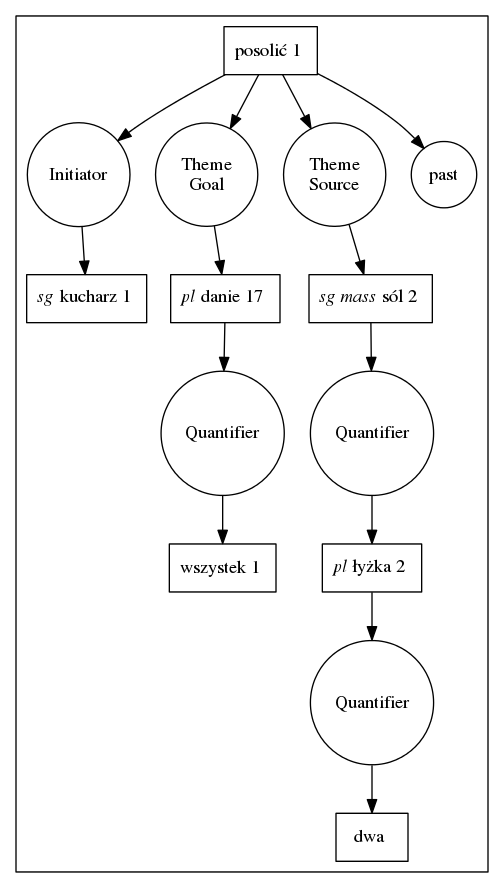
\includegraphics[scale=0.3]{metaopis_sol.png}

%za pierwszym/drugim razem, co drugi raz

\section{Partykuły przyrematyczne i nieprawdomówne, podmiot epistemiczny}
Możemy wyróżnić partykuły, których argument semantyczny jest zdeterminowany składniowo,
{\it niejako, niemniej, oby, omalże, zwłaszcza, lada, ledwie, ledwo, nadto,
aż, wprost, akurat, dosyć, dość, wszak, zaledwie, przecież, zaprawdę, zaiste,
dopiero, jeszcze, już, doprawdy, ponadto} 
% są reprezentowane jako predykaty
% przyjmujące zmienną modelową nadrzędnika (czyli identyfikator podformuły wprowadzanej przez ich nadrzędnik):
np {\it Jan lubi arbuzy zwłaszcza zimą}.
Oraz partykuły, których argument semantyczny nie jest rozpoznawalny na poziomie 
opisu składniowego, w szczególności partykuły przyrematyczne 
modyfikujące akcentowaną, potencjalnie odległą część zdania (remat).%, reprezentowane
% są jako modyfikujące całe zdanie. Należy to rozumieć jako niedospecyfikowane 
% wskazanie maksymalnej możliwej podformuły modyfikowanej przez kublik.
Kublikami takimi są {\it otóż, notabene, owszem, prawda, skądinąd,
również, także, też, znowu, znów, zarazem, tylko, niestety, jedynie, wręcz,
naprawdę, oczywiście, naturalnie, wprawdzie, właśnie, nareszcie, wreszcie,
bynajmniej}. 

Niektóre spośród nich, gwarantują prawdziwość modyfikowanego 
modelu w modelu zewnętrznym, w którym same są interpretowane
(partykuły faktywne): %, wprowadzają dodatkowo koniunkt mówiący o faktywności, widoczny w ostatniej linii przykładu:
{\it Anna oczywiście zaśpiewała Marsyliankę.}
Inne (partykuły nieprawdomówne) tworzą niefaktywny kontekst obejmujący fragment zdania,
często jest nim remat.

Partykuły, których zakres argumentu nie jest zadany przez morfoskładnię,
będziemy reprezentować w sposób niedospecyfikowany podobnie jak kwantyfikatory.
%Podobnie postąpimy z nieprawdomównymi przysłówkami.
Np. {\it Słoń prawdopodobnie trąbi}
\[\begin{tikzpicture}
\node[concept] (b) {\sg słoń};
\node[relation, left=1cm of b] (a) {Pres};
\node[relation, right=10mm of b] (c) {Init};
\node[concept, right=10mm of c] (d) {trąbić};
\node[relation, right=10mm of d] (e) {Op};
\node[concept, right=10mm of e] (f) {prawdopodobnie};
\context{cx}{(b)(c)(d)(e)(f)}{};
\edge{c}{b};
\edge{cx}{a};
\edge{d}{c};
\edge{d}{e};
\edge{e}{f};
\end{tikzpicture}\]
Negację traktujemy jako partykułę nieprawdomówną np. {\it Słoń nie trąbi}.
\[\begin{tikzpicture}
\node[concept] (b) {\sg słoń};
\node[relation, left=1cm of b] (a) {Pres};
\node[relation, right=10mm of b] (c) {Init};
\node[concept, right=10mm of c] (d) {trąbić};
\node[relation, right=10mm of d] (e) {Op};
\node[concept, right=10mm of e] (f) {nie};
\context{cx}{(b)(c)(d)(e)(f)}{};
\edge{c}{b};
\edge{cx}{a};
\edge{d}{c};
\edge{d}{e};
\edge{e}{f};
\end{tikzpicture}\]
co możemy w skrócie zapisać jako
\[\begin{tikzpicture}
\node[concept] (b) {\sg słoń};
\node[relation, left=1cm of b] (a) {Pres};
\node[relation, right=10mm of b] (c) {Init};
\node[concept, right=10mm of c] (d) {{\it nie} trąbić};
\context{cx}{(b)(c)(d)}{};
\edge{c}{b};
\edge{cx}{a};
\edge{d}{c};
\end{tikzpicture}\]
%TODO: OPISAĆ
%$\neg\exists$ traktujemy jako całość, a potem jako dwa symbole - ciekawe zjawisko logicznie.
%Fałszywe jabłko nie spadło\\
%Jedno jabłko nie spadło
%Dwa jabłka nie spadły $\pred{Q}(q,\text{dwa})\wedge\pred{type}(j,\text{jabłko}\wedge{restr}(q,j)$
%Po wypadku nie przerwałem pracy\\

%TODO
%Nie wróciłem do Warszawy po wojnie
%nie prawda, że\\
%nie on to zrobił\\
%nie szef to zrobił\\
%bez pieniędzy\\
%nie do domu

%TODO zmiana kwantyfikatorów w zasięgu negacji
%nikt, nigdy, żaden $\to$ każdy, zawsze (poza zasięgiem negacji)\\
%(nie ktoś, kiedyś, (w zasięgu negacji) bo:)\\
%prawie nigdy $\to$ prawie zawsze 

Podobnie zachowują się {\it chyba, także, również, też, nawet, pewnie, może, być może}.

Dodatkowo, gdy wyrażenie odnosi do stanów mentalnych osoby niekoniecznie tożsamej z nadawcą (podmiot epistemiczny)
dodajemy argument {\it pro} wskazujący tą osobę, zjawisko to występuje np. przy leksemach {\it chyba, pewnie, nawet, chociaż, ale, a}.
%\popr{Jak zapisać zdania {\it Słoń już trąbi}, 
{\it Słoń nawet trąbi}
\[\begin{tikzpicture}
\node[concept] (b) {\sg słoń};
\node[relation, left=1cm of b] (a) {Pres};
\node[relation, right=10mm of b] (c) {Init};
\node[concept, right=10mm of c] (d) {trąbić};
\node[relation, right=10mm of d] (e) {Op};
\node[concept, right=10mm of e] (f) {nawet};
\node[relation, right=10mm of f] (g) {Expr};
\node[concept, right=10mm of g] (h) {\ind pro};
\context{cx}{(b)(c)(d)(e)(f)(g)(h)}{};
\edge{c}{b};
\edge{cx}{a};
\edge{d}{c};
\edge{d}{e};
\edge{e}{f};
\edge{f}{g};
\edge{g}{h};
\end{tikzpicture}\]

%TODO Konstrukcje wzmacniające
% {\it dokładnie pięć słoni}
% {\it jeden słoń}

\section{Koordynacja}\label{coordination}
Koordynację reprezentujemy jako kontekst etykietowany spójnikiem, zawierający listę koordynowanych obiektów.
Graficznie kolejność elementów na liście jest wyrażona poprzez ich ułożenie od lewej do prawej.

Użycie kontekstu pozwala wyjść poza domyślną dla grafów pojęć zasadę łączenia poszczególnych węzłów za pomocą koniunkcji, np:
w zdaniu {\it Jaś, Ania lub Marysia śpiewa.} kontekst {\it lub} zostanie zastąpiony w formule logicznej przez alternatywę.
\[\begin{tikzpicture}
\node[concept] (a) {\sg osoba ''Jaś''};
\node[concept, right=5mm of a] (b) {\sg osoba ''Ania''};
\node[concept, right=5mm of b] (c) {\sg osoba ''Marysia''};
\context{v}{(a)(b)(c)}{lub};
\node[relation, right=10mm of c] (d) {Init};
\node[concept, right=10mm of d] (e) {śpiewać};
\node[relation, right=10mm of e] (f) {Pres};
\context{cx}{(v)(d)(e)}{};
\edge{d}{v};
\edge{e}{d};
\edge{cx}{f};
\end{tikzpicture}\]
Współdzielone podrzędniki koordynacji reprezentujemy dodając koreferencyjny niemy zaimek {\it pro}.
Dzięki temu, nie musimy rozstrzygać czy w zdaniu {\it Słoń biegnie i trąbi} trąbiącym jest {\it słoń}.
\[\begin{tikzpicture}
\node[concept] (a) {biec};
\node[relation, below=5mm of a] (b) {Init};
\node[concept, below=5mm of b] (c) {\sg słoń};
\node[relation, below=5mm of c] (g) {Pres};
\context{v}{(a)(b)(c)}{};
\node[concept, right=30mm of a] (d) {trąbić};
\node[relation, below=5mm of d] (e) {Init};
\node[concept, below=5mm of e] (f) {\corf pro-3sg};
\node[relation, below=5mm of f] (h) {Pres};
\context{w}{(d)(e)(f)}{};
\context{cx}{(v)(w)(g)(h)}{i};
\edge{a}{b};
\edge{b}{c};
\edge{v}{g};
\edge{d}{e};
\edge{e}{f};
\edge{w}{h};
\end{tikzpicture}\]
Sekwencje fraz rozdzielone przecinkami, bądź średnikami traktujemy tak jak frazy skoordynowane, np.
{\it Przybyłem, zobaczyłem, zwyciężyłem.}
\[\begin{tikzpicture}
\node[concept] (a) {przybyć};
\node[relation, below=5mm of a] (b) {Init};
\node[concept, below=5mm of b] (c) {\ind pro-ja-m};
\node[relation, below=5mm of c] (g) {Past};
\context{v}{(a)(b)(c)}{};
\node[concept, right=30mm of a] (d) {zobaczyć};
\node[relation, below=5mm of d] (e) {Init};
\node[concept, below=5mm of e] (f) {\ind pro-ja-m};
\node[relation, below=5mm of f] (h) {Past};
\context{w}{(d)(e)(f)}{};
\node[concept, right=30mm of d] (i) {zwyciężyć};
\node[relation, below=5mm of i] (j) {Init};
\node[concept, below=5mm of j] (k) {\ind pro-ja-m};
\node[relation, below=5mm of k] (l) {Past};
\context{u}{(i)(j)(k)}{};
\context{cx}{(v)(w)(u)(g)(h)(l)}{,};
\edge{a}{b};
\edge{b}{c};
\edge{v}{g};
\edge{d}{e};
\edge{e}{f};
\edge{w}{h};
\edge{i}{j};
\edge{j}{k};
\edge{u}{l};
\end{tikzpicture}\]
Sekwencje zdań również reprezentujemy jako koordynację, np.
{\it Przybyłem. Zobaczyłem. Zwyciężyłem.}
\[\begin{tikzpicture}
\node[concept] (a) {przybyć};
\node[relation, below=5mm of a] (b) {Init};
\node[concept, below=5mm of b] (c) {\ind pro-ja-m};
\node[relation, below=5mm of c] (g) {Past};
\context{v}{(a)(b)(c)}{};
\node[concept, right=30mm of a] (d) {zobaczyć};
\node[relation, below=5mm of d] (e) {Init};
\node[concept, below=5mm of e] (f) {\ind pro-ja-m};
\node[relation, below=5mm of f] (h) {Past};
\context{w}{(d)(e)(f)}{};
\node[concept, right=30mm of d] (i) {zwyciężyć};
\node[relation, below=5mm of i] (j) {Init};
\node[concept, below=5mm of j] (k) {\ind pro-ja-m};
\node[relation, below=5mm of k] (l) {Past};
\context{u}{(i)(j)(k)}{};
\context{cx}{(v)(w)(u)(g)(h)(l)}{.};
\edge{a}{b};
\edge{b}{c};
\edge{v}{g};
\edge{d}{e};
\edge{e}{f};
\edge{w}{h};
\edge{i}{j};
\edge{j}{k};
\edge{u}{l};
\end{tikzpicture}\]

Leksemy spójników złożonych reprezentujemy umieszczając ``\dots'' w polach poszczególnych argumentów, np.:
{\it zarówno słoń jak i żyrafa}. Argumenty występują na liście w kolejności takiej jak ich pola.
\[\begin{tikzpicture}
\node[concept] (a) {\sg słoń};
\node[concept, right=5mm of a] (b) {\sg żyrafa};
\context{v}{(a)(b)}{zarówno \dots{} jak i \dots};
\end{tikzpicture}\]

Spójniki współrzędne niosą znaczenie ``i'' oraz ``lub'' na poziomie zwykłej logiki uzupełnione o wkład metatekstowy.
Te, które mają znaczenie ``i'' mogą zachowywać się addytywnie bądź multiplikatywnie.
Powyższa reprezentacja nie wskazuje tych dwu znaczeń oraz pozostawia addytywność i multiplikatywność niedospecyfikowaną.

Poszczególne użycia spójnika ``i'' oraz innych spójników mających jego znaczenie można przetłumaczyć na reprezentację 
nie zawierających jawnego wystąpienia spójnika, np: kontekst wprowadzany przez przecinek sygnalizujący następstwo zdarzeń w zdaniu
{\it Przybyłem, zobaczyłem, zwyciężyłem.} możemy przetłumaczyć na
\[\begin{tikzpicture}
\node[concept] (a) {przybyć};
\node[relation, below=5mm of a] (b) {Init};
\node[concept, below=5mm of b] (c) {\ind pro-ja-m};
\node[relation, below=5mm of c] (g) {Past};
\node[relation, right=16mm of b] (m) {Succ};
\context{v}{(a)(b)(c)}{};
\node[concept, right=35mm of a] (d) {zobaczyć};
\node[relation, below=5mm of d] (e) {Init};
\node[concept, below=5mm of e] (f) {\ind pro-ja-m};
\node[relation, below=5mm of f] (h) {Past};
\context{w}{(d)(e)(f)}{};
\node[relation, right=16mm of e] (n) {Succ};
\node[concept, right=35mm of d] (i) {zwyciężyć};
\node[relation, below=5mm of i] (j) {Init};
\node[concept, below=5mm of j] (k) {\ind pro-ja-m};
\node[relation, below=5mm of k] (l) {Past};
\context{u}{(i)(j)(k)}{};
\edge{a}{b};
\edge{b}{c};
\edge{v}{g};
\edge{d}{e};
\edge{e}{f};
\edge{w}{h};
\edge{i}{j};
\edge{j}{k};
\edge{u}{l};
\edge{v}{m};
\edge{m}{w};
\edge{w}{n};
\edge{n}{u};
\end{tikzpicture}\]
Zdanie {\it Myślę, więc jestem} z mającym wkład metatekstowy spójnikiem {\it więc} możemy zapisać na następujące sposoby:
\[\begin{tikzpicture}
\node[concept] (a) {myśleć};
\node[relation, below=5mm of a] (b) {Init};
\node[concept, below=5mm of b] (c) {\ind pro-ja};
\node[relation, below=5mm of c] (g) {Pres};
\context{v}{(a)(b)(c)}{};
\node[concept, right=35mm of a] (d) {być};
\node[relation, below=5mm of d] (e) {Thme};
\node[concept, below=5mm of e] (f) {\ind pro-ja};
\node[relation, below=5mm of f] (h) {Pres};
\context{w}{(d)(e)(f)}{};
\context{cx}{(v)(w)(g)(h)}{więc};
\edge{a}{b};
\edge{b}{c};
\edge{v}{g};
\edge{d}{e};
\edge{e}{f};
\edge{w}{h};
\end{tikzpicture}\]
\[\begin{tikzpicture}
\node[concept] (a) {myśleć};
\node[relation, below=5mm of a] (b) {Init};
\node[concept, below=5mm of b] (c) {\ind pro-ja};
\node[relation, below=5mm of c] (g) {Pres};
\context{v}{(a)(b)(c)}{};
\node[concept, right=45mm of a] (d) {być};
\node[relation, below=5mm of d] (e) {Thme};
\node[concept, below=5mm of e] (f) {\ind pro-ja};
\node[relation, below=5mm of f] (h) {Pres};
\context{w}{(d)(e)(f)}{};
%TODO: czy ta reprezentacja jest sensowna, czy nie lepiej zrobić relację ``więc''
\node[relation, right=18mm of a] (i) {???};
\node[concept, below=5mm of i] (j) {więc};
\node[relation, below=5mm of j] (k) {???};
\edge{a}{b};
\edge{b}{c};
\edge{v}{g};
\edge{d}{e};
\edge{e}{f};
\edge{w}{h};
\edge{v}{i};
\edge{i}{j};
\edge{j}{k};
\edge{k}{w};
\end{tikzpicture}\]

W ramach reprezentacji nie sygnalizujemy dystrybutywności i kolektywności koordynacji.
Przykładowo dla zdania {\it Artur spał w Pile i Spale} nie zaznaczamy, że 
występują dwa miejsca i dwie czynności spania. Jeśli koordynowane podrzędniki wnoszą relacje 
wyciągamy je poza kontekst koordynacji np {\it duży i gruby słoń}, {\it czerwony i niebieski ręcznik}, {\it czarno-biały telewizor}:
\[\begin{tikzpicture}
\node[concept] (a) {duży};%TODO relacyjność
\node[concept, right=5mm of a] (b) {gruby};
\context{v}{(a)(b)}{i};
\node[relation, right=10mm of b] (d) {Attr};
\node[concept, right=10mm of d] (e) {\sg słoń};
\edge{d}{v};
\edge{e}{d};
\end{tikzpicture}\]
\[\begin{tikzpicture}
\node[concept] (a) {czerwony};
\node[concept, right=5mm of a] (b) {niebieski};
\context{v}{(a)(b)}{i};
\node[relation, right=10mm of b] (d) {Attr};
\node[concept, right=10mm of d] (e) {\sg ręcznik};
\edge{d}{v};
\edge{e}{d};
\end{tikzpicture}\]
\[\begin{tikzpicture}
\node[concept] (a) {czarny};
\node[concept, right=5mm of a] (b) {biały};
\context{v}{(a)(b)}{-};
\node[relation, right=10mm of b] (d) {Attr};
\node[concept, right=10mm of d] (e) {\sg telewizor};
\edge{d}{v};
\edge{e}{d};
\end{tikzpicture}\]
W przypadku, gdy człony koordynacji wnoszą różne relacje, nie są intersektywne
lub jeden wnosi relację a drugi nie fraza zostaje przekształcona dystrybutywnie, np: 
{\it prawdziwi czy fałszywi bogowie}:
\[\begin{tikzpicture}
\node[concept] (a) {\pl bóg};
\node[relation, below=5mm of a] (b) {Attr};%TODO: czy taka relacja?
\node[concept, below=5mm of b] (c) {prawdziwy};%TODO: metatekst?
\node[concept, right=15mm of a] (d) {\pl fałszywy(bóg)};
\context{v}{(a)(b)(c)(d)}{czy};
\edge{a}{b};
\edge{b}{c};
\end{tikzpicture}\]
{\it Żyję tu i teraz}:
\[\begin{tikzpicture}
\node[concept] (a) {żyć};
\node[relation, below=5mm of a] (b) {Loc};
\node[concept, below=5mm of b] (c) {\ind tu};
\node[concept, right=15mm of a] (d) {żyć};
\node[relation, below=5mm of d] (e) {Time};
\node[concept, below=5mm of e] (f) {\ind teraz};
\context{v}{(a)(b)(c)(d)(e)(f)}{i};
\node[relation, right=15mm of e] (g) {Thme};
\node[concept, right=10mm of g] (h) {\ind pro-ja};
\context{cx}{(v)(g)(h)}{};
\node[relation, right=10mm of h] (i) {Pres};
\edge{a}{b};
\edge{b}{c};
\edge{d}{e};
\edge{e}{f};
\edge{v}{g};
\edge{g}{h};
\edge{cx}{i};
\end{tikzpicture}\]
Jeśli dodatkowo uznamy, że mamy tu do czynienia z addytywnym {\it i}
możemy usunąć koordynację:
\[\begin{tikzpicture}
\node[concept] (a) {żyć};
\node[relation, left=10mm of a] (b) {Loc};
\node[concept, below=5mm of b] (c) {\ind tu};
\node[relation, below=5mm of a] (e) {Time};
\node[concept, below=5mm of e] (f) {\ind teraz};
\node[relation, right=10mm of a] (g) {Thme};
\node[concept, right=10mm of g] (h) {\ind pro-ja};
\context{cx}{(a)(b)(c)(d)(f)(g)(h)}{};
\node[relation, right=10mm of h] (i) {Pres};
\edge{a}{b};
\edge{b}{c};
\edge{a}{e};
\edge{e}{f};
\edge{a}{g};
\edge{g}{h};
\edge{cx}{i};
\end{tikzpicture}\]
%{\it liście dębów i grabów} (do tego trzeba najpierw zrobić Poss)
%koordynacja podtrzędników różnych typów (Lubię Piotra i to, że mnie kocha)
%{\it W tej lecznicy usunięto pacjentce martwą ciążę, a także macicę i fragment jelita}

Zredukowane, mające tylko jeden argument spójniki, 
gramatycznie interpretowane jako kubliki 
np. {\it albo, ale, a, bo, chociaż, choć, i, czyli}
reprezentujemy jako koordynację, której drugim argumentem jest {\it pro-zdarzenie}
np. zdanie {\it I trąbi}:
\[\begin{tikzpicture}
\node[concept] (a) {pro-zdarzenie};
\context{v}{(a)}{};
\node[concept, right=30mm of a] (d) {trąbić};
\node[relation, below=5mm of d] (e) {Init};
\node[concept, below=5mm of e] (f) {\corf pro-3sg};
\node[relation, below=5mm of f] (h) {Pres};
\context{w}{(d)(e)(f)}{};
\context{cx}{(v)(w)(g)(h)}{i};
\edge{d}{e};
\edge{e}{f};
\edge{w}{h};
\end{tikzpicture}\]
% {\it I szukaj korka w polu!}, czy {\it I Zula poszła do urny.}

%TODO: argument cluster coordination dla spójnika ``a'' 
%TODO: składnia - szyk V Conj
%TODO: reprezentacje metatekstowości spójników (np. więc)


Wieloargumentowy przyimek {\it między} traktujemy jak przyimek jednoargumentowy,
którego podrzędnikiem jest koordynacja, np. {\it między stołem, krzesłem a pianinem}
\[\begin{tikzpicture}
\node[concept] (a) {\sg stół};
\node[concept, right=5mm of a] (b) {\sg krzesło};
\node[concept, right=5mm of b] (c) {\sg pianino};
\context{v}{(a)(b)(c)}{a};
\node[relation, right=10mm of c] (d) {Loc};
\node[concept, right=10mm of d] (e) {między};
\edge{d}{v};
\edge[dashed]{d}{e};
\end{tikzpicture}\]


\section{Spójniki podrzędne i zaimki względne}
Spójnik {\it jeśli \dots, to \dots} użyty w znaczeniu logicznej implikacji reprezentujemy za pomocą kontekstu np.
{\it Jeśli słońce świeci, to słoń trąbi}
\[\begin{tikzpicture}
\node[concept] (a) {świecić};
\node[relation, below=5mm of a] (b) {Thme};
\node[concept, below=5mm of b] (c) {\sg słońce};
\node[relation, below=5mm of c] (g) {Pres};
\context{v}{(a)(b)(c)}{};
\node[concept, right=15mm of a] (d) {trąbić};
\node[relation, below=5mm of d] (e) {Init};
\node[concept, below=5mm of e] (f) {\sg słoń};
\node[relation, below=5mm of f] (h) {Pres};
\context{w}{(d)(e)(f)}{};
\context{cx}{(v)(w)(g)(h)}{jeśli \dots, to \dots};
\edge{a}{b};
\edge{b}{c};
\edge{v}{g};
\edge{d}{e};
\edge{e}{f};
\edge{w}{h};
\end{tikzpicture}\]
Zdania ze spójnikami podrzędnymi wnoszącymi znaczenie {\it i} możemy zapisać na dwa sposoby, np
{\it Chociaż słońce świeci, słoń trąbi}:
\[\begin{tikzpicture}
\hspace{-30mm}
\node[concept] (a) {świecić};
\node[relation, below=5mm of a] (b) {Thme};
\node[concept, below=5mm of b] (c) {\sg słońce};
\node[relation, below=5mm of c] (g) {Pres};
\context{v}{(a)(b)(c)}{};
\node[concept, right=15mm of a] (d) {trąbić};
\node[relation, below=5mm of d] (e) {Init};
\node[concept, below=5mm of e] (f) {\sg słoń};
\node[relation, below=5mm of f] (h) {Pres};
\context{w}{(d)(e)(f)}{};
\context{cx}{(v)(w)(g)(h)}{{\it e} chociaż \dots, \dots};
\edge{a}{b};
\edge{b}{c};
\edge{v}{g};
\edge{d}{e};
\edge{e}{f};
\edge{w}{h};
\hspace{60mm}
\node[concept] (a) {świecić};
\node[relation, below=5mm of a] (b) {Thme};
\node[concept, below=5mm of b] (c) {\sg słońce};
\node[relation, below=5mm of c] (g) {Pres};
\node[concept, right=10mm of a] (j) {{\it e} chociaż};
\node[relation, below=5mm of j] (k) {Cond};%TODO relacja
\context{v}{(a)(b)(c)}{};
\node[concept, right=30mm of a] (d) {trąbić};
\node[relation, below=5mm of d] (e) {Init};
\node[concept, below=5mm of e] (f) {\sg słoń};
\node[relation, below=5mm of f] (h) {Pres};
\context{w}{(d)(e)(f)}{};
\edge{a}{b};
\edge{b}{c};
\edge{v}{g};
\edge{d}{e};
\edge{e}{f};
\edge{w}{h};
\edge{w}{k};
\edge[dashed]{k}{j};
\edge{k}{v};
\end{tikzpicture}\]

%TODO negacja zdania ndrzędnego uniemożliwia wyrażenie zdania podrzędnego 
%jako modyfikatora orzeczenia zdania nadrzędnego
%Nie pójdę do kina ponieważ jest za późno.

Zaimki względne również mogą generować implikację. Dlatego będziemy reprezentować je jednocześnie za pomocą kontekstu i pojęcia np.
{\it Kto ma krowę, doi ją}
\[\begin{tikzpicture}
\node[concept] (a) {\corf kto};%TODO czy na pewno coreferential???
\node[relation, below=5mm of a] (b) {Init};%TODO relacja
\node[concept, below=5mm of b] (c) {mieć};
\node[relation, below=5mm of c] (d) {Thme};
\node[concept, below=5mm of d] (e) {\sg krowa};
\node[relation, below=5mm of e] (f) {Pres};
\context{v}{(a)(b)(c)(d)(e)}{};
\node[concept, right=15mm of a] (g) {\corf pro-3sg};
\node[relation, below=5mm of g] (h) {Init};
\node[concept, below=5mm of h] (i) {doić};
\node[relation, below=5mm of i] (j) {Thme};
\node[concept, below=5mm of j] (k) {\sg \corf ona};
\node[relation, below=5mm of k] (l) {Pres};
\context{cv}{(a)(b)(c)(d)(e)}{};
\context{cw}{(g)(h)(i)(j)(k)}{};
\context{cx}{(cv)(cw)(f)(l)}{kto \dots, \dots};%TODO a może ``rel''
\edge{b}{a};
\edge{c}{b};
\edge{c}{d};
\edge{d}{e};
\edge{cv}{f};
\edge{h}{g};
\edge{i}{h};
\edge{i}{j};
\edge{j}{k};
\edge{cw}{l};
\end{tikzpicture}\]

% Zdanie {\it Kto jest mężczyzną, nosi brodę} trzeba zinterpretować tak by uzyskać implikację,
% co można uzyskać dzięki zagnieżdżonym typom.

% Zdanie {\it Rolnik, który ma krowę, doi ją} ma raczej egzystencjalną kwantyfikację ``rolnika''.

% Zdania zawierające zdania podrzędne wprowadzone przez zaimek {\it który} są 
% interpretowane tak samo jak zdania zawierające 
% konstrukcje imiesłowowe, np.
{\it Kupiłem filiżankę, która jest ręcznie malowana.}
\[\begin{tikzpicture}
\node[concept] (a) {kupić};
\node[relation, left=1cm of a] (b) {Init};
\node[concept, left=1cm of b] (c) {\ind pro-ja-m};
\node[relation, left=1cm of c] (d) {Past};
\node[relation, right=1cm of a] (e) {Thme};
\node[concept, right=1cm of e] (f) {\sg filiżanka $\ast x$};
\node[concept, below=1cm of b] (h) {malować};
\node[relation, left=1cm of h] (i) {Manner};
\node[concept, left=1cm of i] (j) {ręcznie};
\node[relation, right=1cm of h] (g) {Thme};
\node[concept, right=1cm of g] (k) {\sg \corf który $?x$};
\node[relation, left=1cm of j] (l) {Pres};
\context{cx}{(a)(b)(c)(e)(f)}{};
\context{cy}{(h)(i)(j)(g)(k)}{};
\context{cz}{(d)(cx)(cy)(l)}{\dots, który \dots};
% \node[relation, below=0.8cm of b] (p) {Time};
% \node[concept, right=1cm of p] (q) {czas};
% \node[relation, right=1cm of q] (r) {Time};
\edge {a} {b};
\edge {b} {c};
\edge {cx} {d};
\edge {a} {e};
\edge {e} {f};
\edge {g} {k};
\edge {h} {g};
\edge {h} {i};
\edge {i} {j};
\edge {cy} {l};
% \edge {cx} {p};
% \edge {p} {q};
% \edge {cy} {r};
% \edge {r} {q};
\end{tikzpicture}\]

\section{Dalsze zagadnienia dotyczące koordynacji}
\begin{itemize}
\item zakres koordynacji a zakres kwantyfikacji {\it nie tylko \dots, ale i \dots} {\it Oceniano nie tylko słowa, ale i głos}
\item kompozycjonalność frazy koordynowanej,
interpretacja ``nie'' w konstrukcjach ``nie ... a ...'', ``nie ... ani ...''.
\item interakcja koordynacji i koreferencji przy spójniku {\it jeśli}, (zamiana kwantyfikatorów z egzystencjalnych na uniwersalne)
\item koordynacja czasowników zanegowanych {\it Jan nie odpowiedział i wyszedł}
\item  Co zrobić przy koordynacji różnych kwantyfikatorów {\it Wszystkie słonie i niektóre samochody zatrąbiły}, czyli
tak jak w zdaniu Hintikki (Za: Jakub Szymanik ``PROBLEMY Z FORMĄ LOGICZNĄ''): 
{\it Pewien krewniak każdego wieśniaka i pewien krewniak każdego mieszczucha nienawidzą się nawzajem};
{\it Większość krewniaków każdego wieśniaka i większość krewniaków każdego mieszczucha nienawidzi się nawzajem}.
\item Jak wyrazić 'wkład meta językowy', czyli odróżnić {\it Jan tańczy i śpiewa} od {\it Jan tańczy, ale i śpiewa};
jak wyrazić sekwencyjne 'i' {\it Jan wstał i poszedł}
\end{itemize}

\section{Wewnętrzne modele}
Zdanie, które jest przedmiotem przekonań, pragnień, komunikacji nie musi być obiektywnie prawdziwe.
Umieszczamy je w pudełku oznaczającym, że jego prawdziwość należy określać ze względu na subiektywny model świata, np {\it 
Jan wierzy, że słoń trąbi.}
% \[\begin{tikzpicture}
% \node[concept] (b) {wierzyć};
% \node[relation, left=10mm of b] (c) {Init};
% \node[concept, left=10mm of c] (d) {\sg osoba ''Jan''};
% \node[relation, right=10mm of b] (e) {że};
% \node[concept, right=10mm of e] (f) {trąbić};
% \node[relation, right=10mm of f] (g) {Init};
% \node[concept, right=10mm of g] (h) {\sg słoń};
% \context{v}{(f)(g)(h)}{};
% \edge{b}{c};
% \edge{c}{d};
% \edge{b}{e};
% \edge{e}{v};
% \edge{f}{g};
% \edge{g}{h};
% \context{cx}{(a)(b)(c)(d)(e)(f)(g)(h)(v)}{};
% \end{tikzpicture}\]
% alternatywnie
\[\begin{tikzpicture}
\node[concept] (b) {wierzyć};
\node[relation, left=10mm of b] (c) {Expr};
\node[concept, left=10mm of c] (d) {\sg osoba ''Jan''};
\node[relation, right=10mm of b] (e) {Thme};
\node[concept, right=10mm of e] (f) {trąbić};
\node[relation, right=10mm of f] (g) {Init};
\node[concept, right=10mm of g] (h) {\sg słoń};
\context{v}{(f)(g)(h)}{};
\edge{b}{c};
\edge{c}{d};
\edge{b}{e};
\edge{e}{v};
\edge{f}{g};
\edge{g}{h};
\context{cx}{(a)(b)(c)(d)(e)(f)(g)(h)(v)}{};
\end{tikzpicture}\]
Podobnie jak przyimki, spójniki podrzędne dzielimy na semantyczne i niesemantyczne,
zgodnie z tym, co stanowi o nich {\it Walenty}. Spójniki niesemantyczne 
nie są odzwierciedlane w grafach semantycznych.

Mowa niezależna i zależna są interpretowane w sposób maksymalnie zbliżony, 
np. {\it Jaś zawołał, że chce jeść}
\[\begin{tikzpicture}
\node[concept] (b) {zawołać};
\node[relation, left=10mm of b] (c) {Init};
\node[concept, left=10mm of c] (d) {\sg osoba ''Jaś''};
\node[relation, right=10mm of b] (e) {Thme};
\node[concept, below=12mm of b] (f) {chcieć};
\node[relation, left=10mm of f] (g) {Init};
\node[concept, left=10mm of g] (h) {\corf pro-3sg};
\node[relation, right=10mm of f] (i) {Thme};
\node[concept, below=12mm of f] (j) {jeść};
\node[relation, left=10mm of j] (k) {Init};
\node[concept, left=10mm of k] (l) {\corf pro};
\node[relation, left=35mm of d] (a) {Past};
\node[relation, left=10mm of h] (m) {Pres};
\context{cv}{(j)(k)(l)}{};
\context{cw}{(f)(g)(h)(i)(cv)}{};
\context{cx}{(b)(c)(d)(e)(cw)(m)}{};
\edge{b}{c};
\edge{c}{d};
\edge{b}{e};
\edge{e}{cw};
\edge{f}{g};
\edge{g}{h};
\edge{f}{i};
\edge{i}{cv};
\edge{j}{k};
\edge{k}{l};
\edge{cx}{a};
\edge{cw}{m};
\end{tikzpicture}\]
oraz {\it - Chcę jeść - zawołał Jaś}
\[\begin{tikzpicture}
\node[concept] (b) {zawołać};
\node[relation, left=10mm of b] (c) {Init};
\node[concept, left=10mm of c] (d) {\sg osoba ''Jaś''};
\node[relation, right=10mm of b] (e) {Thme};
\node[concept, below=12mm of b] (f) {chcieć};
\node[relation, left=10mm of f] (g) {Init};
\node[concept, left=10mm of g] (h) {\ind pro-ja};
\node[relation, right=10mm of f] (i) {Thme};
\node[concept, below=12mm of f] (j) {jeść};
\node[relation, left=10mm of j] (k) {Init};
\node[concept, left=10mm of k] (l) {\corf pro};
\node[relation, left=30mm of d] (a) {Past};
\node[relation, left=10mm of h] (m) {Pres};
\context{cv}{(j)(k)(l)}{};
\context{cw}{(f)(g)(h)(i)(cv)}{};
\context{cx}{(b)(c)(d)(e)(cw)(m)}{};
\edge{b}{c};
\edge{c}{d};
\edge{b}{e};
\edge{e}{cw};
\edge{f}{g};
\edge{g}{h};
\edge{f}{i};
\edge{i}{cv};
\edge{j}{k};
\edge{k}{l};
\edge{cx}{a};
\edge{cw}{m};
\end{tikzpicture}\]
Kiedy w mowie niezależnej mówca nie jest wskazany dodajemy go oraz zdarzenie komunikowania do reprezentacji logicznej, np. {\it - Chcę jeść}
\[\begin{tikzpicture}
\node[concept] (b) {pro-komunikować};
\node[relation, left=10mm of b] (c) {Init};
\node[concept, left=10mm of c] (d) {\corf pro};
\node[relation, right=10mm of b] (e) {Thme};
\node[concept, below=12mm of b] (f) {chcieć};
\node[relation, left=10mm of f] (g) {Init};
\node[concept, left=10mm of g] (h) {\ind pro-ja};
\node[relation, right=10mm of f] (i) {Thme};
\node[concept, below=12mm of f] (j) {jeść};
\node[relation, left=10mm of j] (k) {Init};
\node[concept, left=10mm of k] (l) {\corf pro};
\node[relation, left=15mm of d] (a) {Past};
\node[relation, left=10mm of h] (m) {Pres};
\context{cv}{(j)(k)(l)}{};
\context{cw}{(f)(g)(h)(i)(cv)}{};
\context{cx}{(b)(c)(d)(e)(cw)(m)}{};
\edge{b}{c};
\edge{c}{d};
\edge{b}{e};
\edge{e}{cw};
\edge{f}{g};
\edge{g}{h};
\edge{f}{i};
\edge{i}{cv};
\edge{j}{k};
\edge{k}{l};
\edge{cx}{a};
\edge{cw}{m};
\end{tikzpicture}\]

Mowę niezależną składającą się z wielu zdań reprezentujemy jako koordynację, np.
{\it - Przybyłem - powiedział Cezar. - Zobaczyłem. Zwyciężyłem.}
\[\begin{tikzpicture}
\node[concept] (m) {powiedzieć};
\node[relation, left=10mm of m] (n) {Init};
\node[concept, left=10mm of n] (o) {\sg osoba ''Cezar''};
\node[relation, right=10mm of m] (p) {Thme};
\node[relation, above=10mm of m] (q) {Past};
\node[concept, below=15mm of o] (a) {przybyć};
\node[relation, below=5mm of a] (b) {Init};
\node[concept, below=5mm of b] (c) {\ind pro-ja-m};
\node[relation, below=5mm of c] (g) {Past};
\context{v}{(a)(b)(c)}{};
\node[concept, right=30mm of a] (d) {zobaczyć};
\node[relation, below=5mm of d] (e) {Init};
\node[concept, below=5mm of e] (f) {\ind pro-ja-m};
\node[relation, below=5mm of f] (h) {Past};
\context{w}{(d)(e)(f)}{};
\node[concept, right=30mm of d] (i) {zwyciężyć};
\node[relation, below=5mm of i] (j) {Init};
\node[concept, below=5mm of j] (k) {\ind pro-ja-m};
\node[relation, below=5mm of k] (l) {Past};
\context{u}{(i)(j)(k)}{};
\context{cx}{(v)(w)(u)(g)(h)(l)}{.};
\context{cy}{(cx)(m)(n)(o)(p)(r)}{};
\edge{m}{n};
\edge{n}{o};
\edge{m}{p};
\edge{p}{cx};
\edge{cy}{q};
\edge{a}{b};
\edge{b}{c};
\edge{v}{g};
\edge{d}{e};
\edge{e}{f};
\edge{w}{h};
\edge{i}{j};
\edge{j}{k};
\edge{u}{l};
\end{tikzpicture}\]

%TODO zależności czasowe między zdaniem podrzędnym a nadrzędnym
% Następujące przykłady ilustrują zależności czasowe między zdaniem podrzędnym a nadrzędnym:
% {\it Pomyślałem}, {\it Pomyślę}, {\it Myślałem, że pomyślałem}, {\it Myślałem, że pomyślę}.
%TODO: grafy

Pytania zadane wprost oraz wyrażone w mowie zależnej interpretujemy umieszczając je w wewnętrznym 
kontekście oraz nadając zaimkowi pytającemu symbol \interr, %TODO co on właściwie znaczy
np: {\it - Kto trąbi?}, {\it Wiem, kto trąbi.}
\[\begin{tikzpicture}
\node[concept] (b) {pro-pytać};
\node[relation, left=10mm of b] (c) {Init};
\node[concept, left=10mm of c] (d) {\corf pro};
\node[relation, right=10mm of b] (e) {Thme};
\node[concept, below=12mm of b] (f) {trąbić};
\node[relation, left=10mm of f] (g) {Init};
\node[concept, left=10mm of g] (h) {\interr kto};
\node[relation, left=25mm of d] (a) {Pres};
\node[relation, left=10mm of h] (m) {Pres};
\context{cw}{(f)(g)(h)}{};
\context{cx}{(b)(c)(d)(e)(cw)(m)}{};
\edge{b}{c};
\edge{c}{d};
\edge{b}{e};
\edge{e}{cw};
\edge{f}{g};
\edge{g}{h};
\edge{cx}{a};
\edge{cw}{m};
\end{tikzpicture}\]
\[\begin{tikzpicture}
\node[concept] (b) {wiedzieć};
\node[relation, left=10mm of b] (c) {Init};
\node[concept, left=10mm of c] (d) {\ind pro-ja};
\node[relation, right=10mm of b] (e) {Thme};
\node[concept, below=12mm of b] (f) {trąbić};
\node[relation, left=10mm of f] (g) {Init};
\node[concept, left=10mm of g] (h) {\interr kto};
\node[relation, left=30mm of d] (a) {Pres};
\node[relation, left=10mm of h] (m) {Pres};
\context{cw}{(f)(g)(h)}{};
\context{cx}{(b)(c)(d)(e)(cw)(m)}{};
\edge{b}{c};
\edge{c}{d};
\edge{b}{e};
\edge{e}{cw};
\edge{f}{g};
\edge{g}{h};
\edge{cx}{a};
\edge{cw}{m};
\end{tikzpicture}\]

Faktywność możemy uwzględnić etykietując konteksty relacją wskazującą,
czy treść kontekstu musi być prawdziwa w kontekście zewnętrznym.
%TODO ukonkretnić i pokazać przykłady
%{\it Jan wie, że pada}
%{\it Janowi wydaje się, że pada}

Tryb przypuszczający zaznacza, że sytuacja nie ma miejsca w rzeczywistości, czyli czyni ją niefaktywną.
Oznaczamy to jednoargumentową relacją Cond.
{\it Zjadłbym słonia.}
\[\begin{tikzpicture}
\node[concept] (a) {zjeść};
\node[relation, left=10mm of a] (b) {Init};
\node[concept, left=10mm of b] (c) {\ind pro-ja-m};
\node[relation, right=10mm of a] (d) {Thme};
\node[concept, right=10mm of d] (e) {\sg słoń};
\node[relation, left=10mm of c] (f) {Cond};
\context{cx}{(a)(b)(c)(d)(e)}{};
\edge{a}{b};
\edge{b}{c};
\edge{a}{d};
\edge{d}{e};
\edge{cx}{f};
\end{tikzpicture}\]
W przyszłości można zastąpić relację Cond poszczególnymi użyciami trybu przypuszczającego, np. 
wyrażeniem intencji.

%TODO problem czasu i trybu przypuszczającego w zdaniach podrzędnych
{\it Stanisław zawołał Franciszka i powiedział, żeby jadł}

\section{Niedenotatywne funkcje języka}
Semantykę trybu rozkazującego definiujemy przez sprowadzenie do mowy zależnej, np. {\it - Jedz!} przetłumaczymy na {\it Nakazał mu jeść}
\[\begin{tikzpicture}
\node[concept] (b) {pro-nakazywać};
\node[relation, left=10mm of b] (c) {Init};
\node[concept, left=10mm of c] (d) {\corf pro};
\node[relation, right=10mm of b] (e) {Thme};
\node[concept, below=12mm of b] (f) {jeść};
\node[relation, left=10mm of f] (g) {Init};
\node[concept, left=10mm of g] (h) {\ind pro-ty};
\node[relation, left=10mm of h] (m) {Fut};
\context{cw}{(f)(g)(h)}{};
\context{cx}{(b)(c)(d)(e)(cw)(m)}{};
\edge{b}{c};
\edge{c}{d};
\edge{b}{e};
\edge{e}{cw};
\edge{f}{g};
\edge{g}{h};
\edge{cw}{m};
\end{tikzpicture}\]
%TODO semantyka wykrzyknika
Podobnie semantyka wołacza jest określona przez sprowadzenie do mowy zależnej, np. {\it - Franciszku!} przetłumaczymy na {\it Zawołał Franciszka}
\[\begin{tikzpicture}
\node[concept] (b) {pro-zawołać};
\node[relation, left=10mm of b] (c) {Init};
\node[concept, left=10mm of c] (d) {\corf pro};
\node[relation, right=10mm of b] (e) {Thme};%TODO rola Rcpt?
\node[concept, right=10mm of e] (f) {\sg osoba ``Franciszek''};
\context{cx}{(b)(c)(d)(e)(f)}{};
\edge{b}{c};
\edge{c}{d};
\edge{b}{e};
\edge{e}{f};
\end{tikzpicture}\]
Połączenie wołacza i trybu rozkazującego daje następującą reprezentację {\it - Franciszku, jedz!}
\[\begin{tikzpicture}
\node[concept] (b1) {pro-zawołać};
\node[relation, left=10mm of b1] (c1) {Init};
\node[concept, left=10mm of c1] (d1) {\corf pro};
\node[relation, right=10mm of b1] (e1) {Thme};
\node[concept, right=10mm of e1] (f1) {\sg osoba ``Franciszek''};
\context{cx1}{(b1)(c1)(d1)(e1)(f1)}{};
\edge{b1}{c1};
\edge{c1}{d1};
\edge{b1}{e1};
\edge{e1}{f1};
\node[concept, below=10mm of e1] (b) {pro-nakazywać};
\node[relation, left=10mm of b] (c) {Init};
\node[concept, left=10mm of c] (d) {\corf pro};
\node[relation, right=10mm of b] (e) {Thme};
\node[concept, below=12mm of b] (f) {jeść};
\node[relation, left=10mm of f] (g) {Init};
\node[concept, left=10mm of g] (h) {\ind pro-ty};
\node[relation, left=10mm of h] (m) {Fut};
\context{cw}{(f)(g)(h)}{};
\context{cx}{(b)(c)(d)(e)(cw)(m)}{};
\edge{b}{c};
\edge{c}{d};
\edge{b}{e};
\edge{e}{cw};
\edge{f}{g};
\edge{g}{h};
\edge{cw}{m};
\context{cz}{(cx1)(cx)}{,};
\end{tikzpicture}\]
{\it - Franciszku, jedz! - powiedział Stanisław.} tłumaczymy na {\it Stanisław zawołał Franciszka i powiedział, żeby jadł}
\[\begin{tikzpicture}
\node[concept] (b1) {pro-zawołać};
\node[relation, left=10mm of b1] (c1) {Init};
\node[concept, left=10mm of c1] (d1) {\sg osoba ``Stanisław''};
\node[relation, right=10mm of b1] (e1) {Thme};
\node[concept, right=10mm of e1] (f1) {\sg osoba ``Franciszek''};
\context{cx1}{(b1)(c1)(d1)(e1)(f1)}{};
\edge{b1}{c1};
\edge{c1}{d1};
\edge{b1}{e1};
\edge{e1}{f1};
\node[concept, below=10mm of e1] (b) {powiedzieć};
\node[relation, left=10mm of b] (c) {Init};
\node[concept, left=10mm of c] (d) {\sg osoba ``Stanisław''};
\node[relation, right=10mm of b] (e) {Thme};
\node[concept, below=12mm of b] (f) {jeść};
\node[relation, left=10mm of f] (g) {Init};
\node[concept, left=10mm of g] (h) {\ind pro-ty};
\node[relation, left=10mm of h] (m) {Fut};
\node[concept, right=10mm of f] (o) {żeby};
\context{cw}{(f)(g)(h)}{};
\context{cx}{(b)(c)(d)(e)(cw)(m)(o)}{};
\edge{b}{c};
\edge{c}{d};
\edge{b}{e};
\edge{f}{g};
\edge{g}{h};
\edge{cw}{m};
\context{cz}{(cx1)(cx)}{,};
\edge[dashed]{e}{o};
\edge{e}{cw};
\end{tikzpicture}\]
Alternatywnie można by powyższe zdanie zinterpretować jako {\it Stanisław powiedział Franciszkowi, żeby jadł}
\[\begin{tikzpicture}
\node[relation, right=10mm] (e1) {Rcpt};
\node[concept, right=10mm of e1] (f1) {\sg osoba ``Franciszek''};
\edge{e1}{f1};
\node[concept, below=10mm of e1] (b) {powiedzieć};
\node[relation, left=10mm of b] (c) {Init};
\node[concept, left=10mm of c] (d) {\sg osoba ``Stanisław''};
\node[relation, right=10mm of b] (e) {Thme};
\node[concept, below=12mm of b] (f) {jeść};
\node[relation, left=10mm of f] (g) {Init};
\node[concept, left=10mm of g] (h) {\ind pro-ty};
\node[relation, left=10mm of h] (m) {Fut};
\node[concept, right=10mm of f] (o) {żeby};
\context{cw}{(f)(g)(h)}{};
\context{cx}{(b)(c)(d)(e)(cw)(m)(o)(f1)(e1)}{};
\edge{b}{c};
\edge{c}{d};
\edge{b}{e};
\edge{f}{g};
\edge{g}{h};
\edge{cw}{m};
\edge[dashed]{e}{o};
\edge{e}{cw};
\edge{b}{e1};
\end{tikzpicture}\]
%{\it - Kocham Cię, Dorotko!}

Zdania w bezokoliczniku oznaczające polecenia reprezentujemy analogicznie do trybu rozkazującego, np. {\it - Stać!}
\[\begin{tikzpicture}
\node[concept] (b) {pro-nakazywać};
\node[relation, left=10mm of b] (c) {Init};
\node[concept, left=10mm of c] (d) {\corf pro};
\node[relation, right=10mm of b] (e) {Thme};
\node[concept, below=12mm of b] (f) {stać};
\node[relation, left=10mm of f] (g) {Init};
\node[concept, left=10mm of g] (h) {\ind pro};
\node[relation, left=10mm of h] (m) {Fut};
\context{cw}{(f)(g)(h)}{};
\context{cx}{(b)(c)(d)(e)(cw)(m)}{};
\edge{b}{c};
\edge{c}{d};
\edge{b}{e};
\edge{e}{cw};
\edge{f}{g};
\edge{g}{h};
\edge{cw}{m};
\end{tikzpicture}\]
%TODO: inne użycia bezokolicznika {\it Błądzić jest rzeczą ludzką}

Wykrzykniki odnoszą do zdarzeń, dlatego reprezentujemy je analogicznie do czasowników  i nadajemy kontekst sytuacyjny, np {\it Para buch, koła w ruch}
\[\begin{tikzpicture}
\node[concept] (b) {buch};
\node[relation, left=10mm of b] (c) {Init};
\node[concept, left=10mm of c] (d) {para};
\node[concept, below=12mm of b] (f) {pro-zdarzenie};
\node[relation, left=10mm of f] (g) {Init};
\node[concept, left=10mm of g] (h) {\pl koło};
\node[relation, right=10mm of f] (i) {Thme};
\node[concept, below=5mm of i] (j) {w};
\node[concept, right=10mm of i] (l) {ruch};
\context{cx}{(b)(c)(d)}{};
\context{cy}{(f)(g)(h)(i)(j)(l)}{};
\context{cz}{(cx)(cy)}{,};
\edge{b}{c};
\edge{c}{d};
\edge{f}{i};
\edge[dashed]{i}{j};
\edge{f}{g};
\edge{g}{h};
\edge{i}{l};
\end{tikzpicture}\]
Znaczenie leksemu {\it buch} możemy zdefiniować jako {\it wydać dźwięk ``buch''}. Pozwoli nam to zapisać frazę {\it Para buch} jako {\it Para wydała dźwięk ``buch''} i reprezentować ją jako:
\[\begin{tikzpicture}
\node[concept] (a) {wydać dźwięk};
\node[relation, left=10mm of a] (b) {Init};
\node[concept, left=10mm of b] (c) {para};
\node[relation, right=10mm of a] (d) {Thme};
\node[concept, right=10mm of d] (e) {dźwięk ``buch''};
\context{cx}{(a)(b)(c)(d)(e)}{};
\edge{a}{b};
\edge{b}{c};
\edge{a}{d};
\edge{d}{e};
\end{tikzpicture}\]
W powyższym grafie {\it wydać dźwięk} jest sensem ze Słowosieci, a {\it dźwięk ``buch''} wygenerowanym dźwiękiem. 
Analogicznie możemy reprezentować pozostałe onomatopeje (np {\it miau, brzdęk, brr, be, baś, brrum, bum, cip-cip}).
Zakładamy, że dla każdego zdarzenia sygnalizowanego przez onomatopeje istnieje jego Initiator.
%Onomatopeje to zdarzenia wystąpienia dźwięku o brzmieniu podobnym do brzmienia leksemu.
Frazę {\it bardzo przymilne miau} zapiszemy jako
\[\begin{tikzpicture}
\node[concept] (b) {miau};
\node[relation, right=10mm of b] (c) {Manr};
\node[concept, right=10mm of c] (d) {przymilny};
\node[relation, right=10mm of d] (e) {Manr};
\node[concept, right=10mm of e] (f) {bardzo};
\edge{b}{c};
\edge{c}{d};
\edge{d}{e};
\edge{e}{f};
\end{tikzpicture}\]
co jest równoważne:
\[\begin{tikzpicture}
\node[concept] (a) {wydać dźwięk};
\node[relation, right=10mm of a] (b) {Thme};
\node[concept, right=10mm of b] (c) {dźwięk ``miau''};
\node[relation, right=10mm of c] (d) {Attr};
\node[concept, right=10mm of d] (e) {przymilny};
\node[relation, right=10mm of e] (f) {Manr};
\node[concept, right=10mm of f] (g) {bardzo};
\edge{a}{b};
\edge{b}{c};
\edge{c}{d};
\edge{d}{e};
\edge{e}{f};
\edge{f}{g};
\end{tikzpicture}\]
Z kolei zdanie {\it A kot z bólu: miau} zinterpretujemy  
tak jak mowę niezależną:
\[\begin{tikzpicture}
\node[concept] (b) {pro-zdarzenie};
\node[relation, left=10mm of b] (c) {Init};
\node[concept, left=10mm of c] (d) {\sg kot};
\node[relation, right=10mm of b] (e) {Cond};
\node[concept, above=5mm of e] (f) {z};
\node[concept, right=10mm of e] (h) {\sg ból};
\node[relation, below=10mm of b] (k) {Thme};
\node[concept, right=10mm of k] (l) {miau};
\node[relation, right=10mm of l] (m) {Init};
\node[concept, right=10mm of m] (n) {\corf pro};
\context{cx}{(l)(m)(n)}{};
\context{cy}{(c)(b)(d)(e)(f)(h)(k)(cx)}{};
\edge{b}{c};
\edge{c}{d};
\edge{b}{e};
\edge[dashed]{e}{f};
\edge{e}{h};
\edge{b}{k};
\edge{k}{cx};
\edge{l}{m};
\edge{m}{n};
\end{tikzpicture}\]
Następnie po rozwiązaniu koreferencji pomiędzy {\it pro-zdarzenie} i {\it miau} otrzymamy
\[\begin{tikzpicture}
\node[concept] (b) {miau};
\node[relation, left=10mm of b] (c) {Init};
\node[concept, left=10mm of c] (d) {\sg kot};
\node[relation, right=10mm of b] (e) {Cond};
\node[concept, above=5mm of e] (f) {z};
\node[concept, right=10mm of e] (h) {\sg ból};
\context{cy}{(c)(b)(d)(e)(f)(h)}{};
\edge{b}{c};
\edge{c}{d};
\edge{b}{e};
\edge[dashed]{e}{f};
\edge{e}{h};
\end{tikzpicture}\]
a po rozwinięciu {\it miau}:
\[\begin{tikzpicture}
\node[concept] (b) {wydać dźwięk};
\node[relation, left=10mm of b] (c) {Init};
\node[concept, left=10mm of c] (d) {\sg kot};
\node[relation, right=10mm of b] (e) {Cond};
\node[concept, above=5mm of e] (f) {z};
\node[concept, right=10mm of e] (h) {\sg ból};
\node[relation, below=10mm of b] (k) {Thme};
\node[concept, right=10mm of k] (l) {dźwięk ``miau''};
\context{cy}{(c)(b)(d)(e)(f)(h)(k)(l)}{};
\edge{b}{c};
\edge{c}{d};
\edge{b}{e};
\edge[dashed]{e}{f};
\edge{e}{h};
\edge{b}{k};
\edge{k}{l};
\end{tikzpicture}\]
Z wykrzyknikami wyrażającymi uczucia i emocje np {\it hurra, fuj, ojejej} związane są osoby, które ich doświadczają, np
{\it Teraz mi się dopiero, ojejej, przypomniało}
\[\begin{tikzpicture}
\node[concept] (a) {przypomnieć się};
\node[relation, left=10mm of a] (b) {Init};
\node[concept, left=10mm of b] (c) {{\it pri} \ind pro};
\node[relation, right=10mm of a] (d) {Time};
\node[concept, right=10mm of d] (e) {\ind teraz};
\node[relation, below=5mm of a] (f) {Manr};%TODO relacja
\node[concept, right=10mm of f] (g) {{\it relational} dopiero};
\node[concept, below=24mm of a] (h) {ojejej};
\node[relation, left=10mm of h] (i) {Expr};
\node[concept, left=10mm of i] (j) {\corf pro};
\node[concept, above=11mm of a] (k) {pro-komunikować};
\node[relation, left=10mm of k] (l) {Init};
\node[concept, left=10mm of l] (m) {\corf pro};
\context{cx}{(a)(b)(c)(d)(e)(f)(g)}{};
\context{cv}{(cx)(k)(l)(m)}{};
\context{cy}{(h)(i)(j)}{};
\context{cz}{(cv)(cy)}{,\dots,}
\edge{a}{b};
\edge{b}{c};
\edge{a}{d};
\edge{d}{e};
\edge{a}{f};
\edge{f}{g};
\edge{h}{i};
\edge{i}{j};
\edge{k}{cx};
\edge{k}{l};
\edge{l}{m};
\end{tikzpicture}\]
W powyższym zdaniu kontekst {\it ,\dots,} oznacza wtrącenie. Z uwagi na metatekstowy charakter {\it ojejej} 
trzeba jawnie wskazać, że {\it Teraz mi się dopiero przypomniało} jest treścią komunikatu.
Możemy zinterpretować {\it ojejej} jako {\it poczuć emocję o nazwie ``ojejej''}.
{\it Emocję ``ojejej''} można potem przetłumaczyć na np. {\it zaskoczenie}.
\[\begin{tikzpicture}
\node[concept] (a) {przypomnieć się};
\node[relation, left=10mm of a] (b) {Init};
\node[concept, left=10mm of b] (c) {{\it pri} \ind pro};
\node[relation, right=10mm of a] (d) {Time};
\node[concept, right=10mm of d] (e) {\ind teraz};
\node[relation, below=5mm of a] (f) {Manr};%TODO relacja
\node[concept, right=10mm of f] (g) {{\it relational} dopiero};
\node[concept, below=24mm of a] (h) {poczuć};%TODO może lepiej: komunikować, tutaj trzeba by zaznaczyć, że emocja jest też komunikowana.
\node[relation, left=10mm of h] (i) {Expr};
\node[concept, left=10mm of i] (j) {\corf pro};
\node[relation, right=10mm of h] (n) {Thme};
\node[concept, right=10mm of n] (o) {emocja ``ojejej''};
\node[concept, above=11mm of a] (k) {pro-komunikować};
\node[relation, left=10mm of k] (l) {Init};
\node[concept, left=10mm of l] (m) {\corf pro};
\context{cx}{(a)(b)(c)(d)(e)(f)(g)}{};
\context{cv}{(cx)(k)(l)(m)}{};
\context{cy}{(h)(i)(j)(n)(o)}{};
\context{cz}{(cv)(cy)}{,\dots,}
\edge{a}{b};
\edge{b}{c};
\edge{a}{d};
\edge{d}{e};
\edge{a}{f};
\edge{f}{g};
\edge{h}{i};
\edge{i}{j};
\edge{k}{cx};
\edge{k}{l};
\edge{l}{m};
\edge{h}{n};
\edge{n}{o};
\end{tikzpicture}\]

Wykrzykniki wyrażające wolę mówiącego (powitania {\it cześć}, kontaktu ze zwierzętami np. {\it kici-kici}), 
apelatywne {\it brawo, uwaga, precz, huzia, jazda, wara, won, a kysz, amen},
parentetyczne {\it halo, ałła, cholera},
potwierdzenia {\it spoko, tak} traktujemy jako zdarzenia, które mają swojego Initiatiora. 
Wykrzykniki te mają charakter trybu rozkazującego, a ich Initiatior to osoba, która wyraża wolę, 
np. %{\it - Amen} można przetłumaczyć na {\it Niech się stanie}, a
{\it - Kici-kici!} można przetłumaczyć na {\it - Kocie podejdź!} i dalej na {\it Nakazał kotu podejść}.
%TODO: czy wszystkie tak się zachowują?
\[\begin{tikzpicture}
\node[concept] (b) {kici-kici};
\node[relation, left=10mm of b] (c) {Init};
\node[concept, left=10mm of c] (d) {\corf pro};
\context{cx}{(b)(c)(d)}{};
\edge{b}{c};
\edge{c}{d};
\end{tikzpicture}\]
\[\begin{tikzpicture}
\node[concept] (b) {pro-nakazywać};
\node[relation, left=10mm of b] (c) {Init};
\node[concept, left=10mm of c] (d) {\corf pro};
\node[relation, right=10mm of b] (e) {Thme};
\node[concept, below=12mm of b] (f) {podejść};
\node[relation, left=10mm of f] (g) {Init};
\node[concept, left=10mm of g] (h) {\ind pro-kot};
\node[relation, left=10mm of h] (m) {Fut};
\context{cw}{(f)(g)(h)}{};
\context{cx}{(b)(c)(d)(e)(cw)(m)}{};
\edge{b}{c};
\edge{c}{d};
\edge{b}{e};
\edge{e}{cw};
\edge{f}{g};
\edge{g}{h};
\edge{cw}{m};
\end{tikzpicture}\]


Emotikony reprezentujemy tak jak wykrzykniki emotywne, {\it Lubię Cię :)}
\[\begin{tikzpicture}
\node[concept] (a) {lubić};
\node[relation, left=10mm of a] (b) {Init};
\node[concept, left=10mm of b] (c) {{\it pri} \ind pro};
\node[relation, right=10mm of a] (d) {Thme};
\node[concept, right=10mm of d] (e) {{\it sec} \ind pro};
\node[concept, below=14mm of a] (h) {:)};
\node[relation, left=10mm of h] (i) {Expr};
\node[concept, left=10mm of i] (j) {\corf pro};
\node[concept, above=11mm of a] (k) {pro-komunikować};
\node[relation, left=10mm of k] (l) {Init};
\node[concept, left=10mm of l] (m) {\corf pro};
\context{cx}{(a)(b)(c)(d)(e)}{};
\context{cv}{(cx)(k)(l)(m)}{};
\context{cy}{(h)(i)(j)}{};
\context{cz}{(cv)(cy)}{,}
\edge{a}{b};
\edge{b}{c};
\edge{a}{d};
\edge{d}{e};
\edge{h}{i};
\edge{i}{j};
\edge{k}{cx};
\edge{k}{l};
\edge{l}{m};
\end{tikzpicture}\]
%TODO a może zaznaczyć, że emotikon odnosi się do komunikatu
Znak wykrzyknienia reprezentujemy podobnie jak emotikony, {\it Lubię Cię!}
\[\begin{tikzpicture}
\node[concept] (a) {lubić};
\node[relation, left=10mm of a] (b) {Init};
\node[concept, left=10mm of b] (c) {{\it pri} \ind pro};
\node[relation, right=10mm of a] (d) {Thme};
\node[concept, right=10mm of d] (e) {{\it sec} \ind pro};
\node[concept, below=14mm of a] (h) {!};
\node[relation, left=10mm of h] (i) {Init};
\node[concept, left=10mm of i] (j) {\corf pro};
\node[concept, above=11mm of a] (k) {pro-komunikować};
\node[relation, left=10mm of k] (l) {Init};
\node[concept, left=10mm of l] (m) {\corf pro};
\context{cx}{(a)(b)(c)(d)(e)}{};
\context{cv}{(cx)(k)(l)(m)}{};
\context{cy}{(h)(i)(j)}{};
\context{cz}{(cv)(cy)}{,}
\edge{a}{b};
\edge{b}{c};
\edge{a}{d};
\edge{d}{e};
\edge{h}{i};
\edge{i}{j};
\edge{k}{cx};
\edge{k}{l};
\edge{l}{m};
\end{tikzpicture}\]
%TODO a może zaznaczyć, że wykrzyknik odnosi się do komunikatu


% Wykrzykniki nie zakwalifikowane do żadnej z powyższych grup, np. cym, ole, ojra, la, na, rym, tralala. Wyrazy te nie mają konkretnego znaczenia i pełnią rolę uzupełniającą. Używane najczęściej jako przyśpiewka w piosenkach.
% Dopowiedzenie {\it aha, ajuści, basta}
% {\it że tak powiem}


\end{document}





\section{Niejednoznaczność}
%TODO OPISAĆ
\begin{center}
{\it Chłód wiatru powiewem ogarnął Jana.}\\
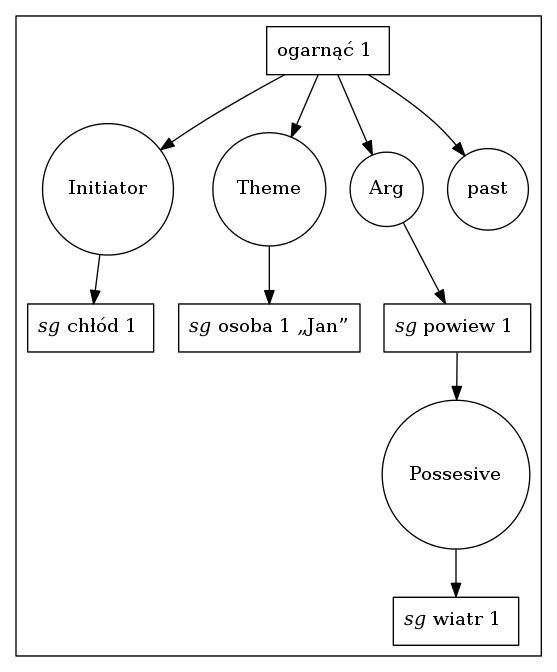
\includegraphics[scale=0.3]{metaopis_wiatr1.png}\\
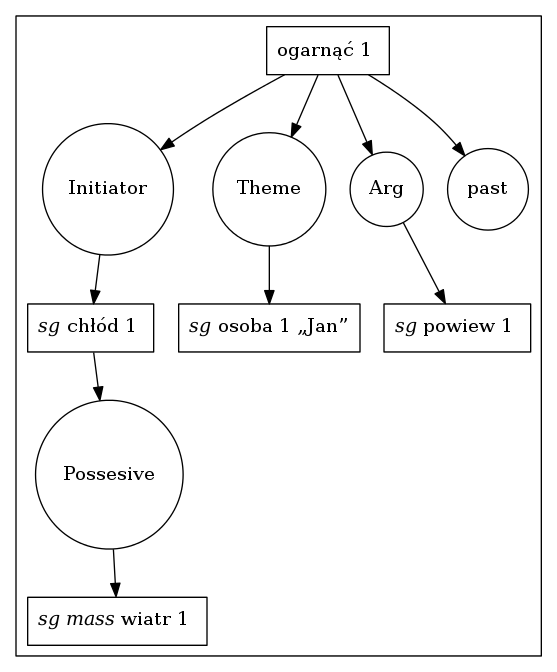
\includegraphics[scale=0.3]{metaopis_wiatr2.png}
\end{center}

\section{Inne przykłady}

% \begin{center}
% Modyfikowany przyimek {\it Ania schowała piłkę głęboko w szafie.}\\
% 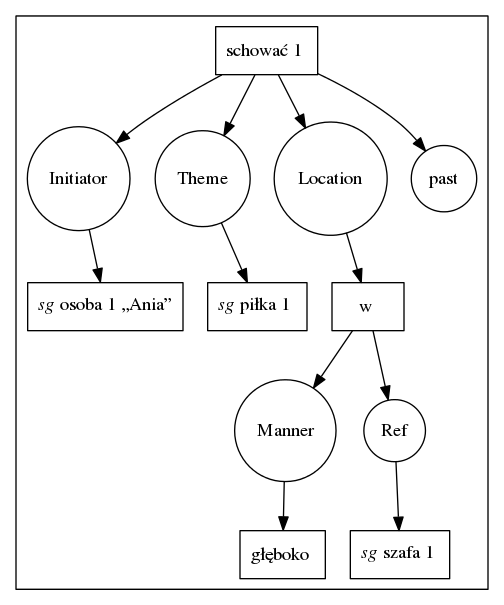
\includegraphics[scale=0.3]{metaopis_gleboko.png}\\
% Role tematyczne, przyimek niesemantyczny {\it Jaś wystosował petycję do urzędu.}\\
% 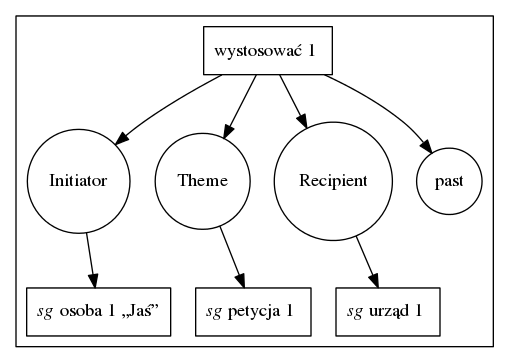
\includegraphics[scale=0.3]{metaopis_wystosowac.png}\\
% Rozpoznanie nazwy własnej dzięki preferencjom selekcyjnym,
% pojemniki i data. 
% {\it Kot odkupił 25 sierpnia 2015 samochód za 20000zł.}\\
% 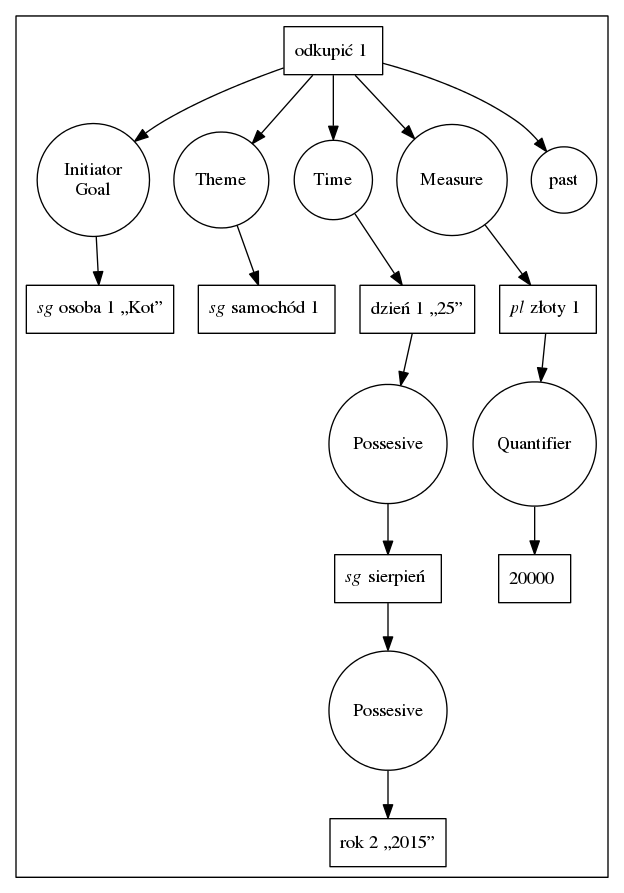
\includegraphics[scale=0.3]{metaopis_odkupic.png}\\
% Wykrycie rzadkiego leksemu, dzięki preferencjom selekcyjnym.
% {\it Chłopcy mają ulicę kwiatami.}\\
% 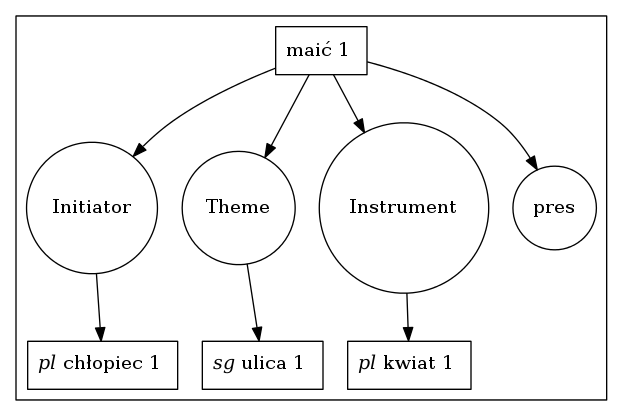
\includegraphics[scale=0.3]{metaopis_maic.png}\\
% Wielopoziomowe konteksty i mowa zależna
% {\it Jaś wierzy, że Marysia kłamała, kiedy powiedziała, że go nie kocha.}\\
% Rzeczowniki odnoszące się do pojęć:
% {\it Słonie są ssakami} vs {\it Słonie są gatunkiem}.\\
% Niejednoznaczność składniowa, kwantyfikator, indexical.
% {\it Codziennie jest tu opiekunka pani Gabrysia}\\
% \end{center}

\section{Zasoby istniejące i wymagające wytworzenia}
%TODO OPISAĆ

Źródła wiedzy: Walenty, informacje składniowe, zasoby semantyczne do utworzenia w Clarin 2
w szczególności kwantyfikatorowatość.

% TODO: niektóre przymiotniki i przysłówki (być może wszystkie)
% warto reprezentować jako leksemy rzeczownikowe, np. lwowsko i
% lwowski jako Lwów.

\end{document}






%uzasadnienie: słownik walencyjny Walenty nie precyzuje kiedy przyimek jest semantyczny, a kiedy nie. 
%Taka reprezentacja powoduje, że uczynienie przyimka niesemantycznym sprowadza się do wykreślenia jego pudełka z grafu.

%Arg

\end{document}